% =====================================================================
% Artigo IEEE (conference, 2 colunas), Equipe 14, PUCPR.
% Compilar: tectonic artigo.tex   (roda o BibTeX e reexecuta sozinho)
% Todo número de resultado vem de numeros.tex (gerado de results/ por
% src/experiments/make_paper_numbers.py; não edite números à mão).
% =====================================================================
\documentclass[conference]{IEEEtran}

\usepackage[utf8]{inputenc}
\usepackage[T1]{fontenc}
\usepackage[brazil]{babel}
\usepackage{graphicx}
\usepackage{booktabs}
\usepackage{amsmath}
\usepackage{multirow}
\usepackage{tabularx}
\usepackage{array}
\usepackage[nocompress]{cite}
\usepackage{xurl}
\usepackage[colorlinks=true,allcolors=black]{hyperref}
\hypersetup{pdftitle={Detecção de Sonolência em Dispositivos Móveis: Avaliação da Generalização entre Sonolência Atuada e Real},
  pdfauthor={André Luís Oliveira Ferreira da Silva, Bruno Rodolfo da Silveira, Bruno Sandoval Ribeiro, Paulo Henrique Perin},
  pdfkeywords={detecção de sonolência, sonolência atuada, sonolência real, generalização entre bases, UTA-RLDD, DMD},
  pdflang={pt-BR}}

% paper/numeros.tex — GERADO por src/experiments/make_paper_numbers.py em 26/10/2026 23:13.
% NÃO EDITE À MÃO: rode `bash tools/atualizar_celular.sh` (ou o script acima).
% Origem de cada número: results/numeros_resumo.md (arquivo, coluna e filtro).
% Percentuais sem o símbolo %; diferenças em pontos percentuais (pp); IC 95% entre colchetes.
\newif\ifSamsungMedido
\SamsungMedidofalse
\newcommand{\SamsungPendente}{medição prevista}
% --- Base ---
\newcommand{\BaseUTASujeitos}{60}
\newcommand{\BaseUTAVideos}{180}
\newcommand{\BaseUTAArquivos}{182}
\newcommand{\BaseUTASequencias}{8.661}
\newcommand{\BaseUTASujeitosOficiais}{58}
\newcommand{\BaseUTAVideosOficiais}{174}
\newcommand{\BaseUTAJanelasBTres}{12.487}
\newcommand{\BaseUTAJanelasSonolentas}{7.581}
\newcommand{\BaseUTAJanelasAlerta}{4.906}
\newcommand{\BaseMRLImagens}{84.898}
\newcommand{\BaseMRLSujeitos}{37}
\newcommand{\BaseCEWImagens}{4.846}
\newcommand{\BaseDMDSujeitos}{13}
\newcommand{\BaseDMDJanelas}{510}
\newcommand{\BaseDMDJanelasSonolentas}{423}
\newcommand{\BaseDMDJanelasAlerta}{87}
\newcommand{\BaseDMDSessoesSonolencia}{16}
\newcommand{\BaseDMDSessoesDirecaoReal}{17}
\newcommand{\BaseDMDSessoes}{65}
\newcommand{\BaseDMDSujeitosTodos}{14}
\newcommand{\BaseNITYMEDVideos}{126}
\newcommand{\BaseNITYMEDMicrossono}{19}
\newcommand{\BaseNITYMEDBocejo}{107}
\newcommand{\BaseNITYMEDDeclarados}{130}
\newcommand{\BaseNITYMEDJanelas}{979}
\newcommand{\BaseNITYMEDJanelasAvaliaveis}{529}
% --- ExpUm ---
\newcommand{\ExpUmRFBSA}{54,5}
\newcommand{\ExpUmRFBSADP}{9,3}
\newcommand{\ExpUmRFBSAMDP}{54,5\,$\pm$\,9,3}
\newcommand{\ExpUmRFAcBal}{57,8}
\newcommand{\ExpUmRFAcBalDP}{7,9}
\newcommand{\ExpUmRFAcBalMDP}{57,8\,$\pm$\,7,9}
\newcommand{\ExpUmRFFMacro}{56,0}
\newcommand{\ExpUmRFFMacroDP}{9,1}
\newcommand{\ExpUmRFFMacroMDP}{56,0\,$\pm$\,9,1}
\newcommand{\ExpUmRFAUC}{73,5}
\newcommand{\ExpUmRFAUCDP}{6,8}
\newcommand{\ExpUmRFAUCMDP}{73,5\,$\pm$\,6,8}
\newcommand{\ExpUmRFVA}{57,3}
\newcommand{\ExpUmRFVADP}{7,2}
\newcommand{\ExpUmRFVAMDP}{57,3\,$\pm$\,7,2}
\newcommand{\ExpUmLSTMBSA}{50,8}
\newcommand{\ExpUmLSTMBSADP}{8,9}
\newcommand{\ExpUmLSTMBSAMDP}{50,8\,$\pm$\,8,9}
\newcommand{\ExpUmLSTMAcBal}{53,1}
\newcommand{\ExpUmLSTMAcBalDP}{6,7}
\newcommand{\ExpUmLSTMAcBalMDP}{53,1\,$\pm$\,6,7}
\newcommand{\ExpUmLSTMFMacro}{51,8}
\newcommand{\ExpUmLSTMFMacroDP}{7,8}
\newcommand{\ExpUmLSTMFMacroMDP}{51,8\,$\pm$\,7,8}
\newcommand{\ExpUmLSTMAUC}{68,6}
\newcommand{\ExpUmLSTMAUCDP}{8,2}
\newcommand{\ExpUmLSTMAUCMDP}{68,6\,$\pm$\,8,2}
\newcommand{\ExpUmLSTMVA}{57,2}
\newcommand{\ExpUmLSTMVADP}{7,5}
\newcommand{\ExpUmLSTMVAMDP}{57,2\,$\pm$\,7,5}
\newcommand{\ExpUmCNNBSA}{48,0}
\newcommand{\ExpUmCNNBSADP}{6,8}
\newcommand{\ExpUmCNNBSAMDP}{48,0\,$\pm$\,6,8}
\newcommand{\ExpUmCNNAcBal}{51,4}
\newcommand{\ExpUmCNNAcBalDP}{5,2}
\newcommand{\ExpUmCNNAcBalMDP}{51,4\,$\pm$\,5,2}
\newcommand{\ExpUmCNNFMacro}{50,0}
\newcommand{\ExpUmCNNFMacroDP}{6,4}
\newcommand{\ExpUmCNNFMacroMDP}{50,0\,$\pm$\,6,4}
\newcommand{\ExpUmCNNAUC}{68,4}
\newcommand{\ExpUmCNNAUCDP}{6,1}
\newcommand{\ExpUmCNNAUCMDP}{68,4\,$\pm$\,6,1}
\newcommand{\ExpUmCNNVA}{55,0}
\newcommand{\ExpUmCNNVADP}{8,2}
\newcommand{\ExpUmCNNVAMDP}{55,0\,$\pm$\,8,2}
\newcommand{\ExpUmSVMBSA}{53,0}
\newcommand{\ExpUmSVMBSADP}{3,8}
\newcommand{\ExpUmSVMBSAMDP}{53,0\,$\pm$\,3,8}
\newcommand{\ExpUmSVMAcBal}{56,2}
\newcommand{\ExpUmSVMAcBalDP}{4,5}
\newcommand{\ExpUmSVMAcBalMDP}{56,2\,$\pm$\,4,5}
\newcommand{\ExpUmSVMFMacro}{54,2}
\newcommand{\ExpUmSVMFMacroDP}{3,9}
\newcommand{\ExpUmSVMFMacroMDP}{54,2\,$\pm$\,3,9}
\newcommand{\ExpUmSVMAUC}{69,9}
\newcommand{\ExpUmSVMAUCDP}{5,1}
\newcommand{\ExpUmSVMAUCMDP}{69,9\,$\pm$\,5,1}
\newcommand{\ExpUmSVMVA}{54,0}
\newcommand{\ExpUmSVMVADP}{4,0}
\newcommand{\ExpUmSVMVAMDP}{54,0\,$\pm$\,4,0}
\newcommand{\ExpUmLRBSA}{49,4}
\newcommand{\ExpUmLRBSADP}{4,3}
\newcommand{\ExpUmLRBSAMDP}{49,4\,$\pm$\,4,3}
\newcommand{\ExpUmLRAcBal}{49,7}
\newcommand{\ExpUmLRAcBalDP}{3,0}
\newcommand{\ExpUmLRAcBalMDP}{49,7\,$\pm$\,3,0}
\newcommand{\ExpUmLRFMacro}{48,5}
\newcommand{\ExpUmLRFMacroDP}{3,6}
\newcommand{\ExpUmLRFMacroMDP}{48,5\,$\pm$\,3,6}
\newcommand{\ExpUmLRAUC}{68,9}
\newcommand{\ExpUmLRAUCDP}{5,5}
\newcommand{\ExpUmLRAUCMDP}{68,9\,$\pm$\,5,5}
\newcommand{\ExpUmLRVA}{50,7}
\newcommand{\ExpUmLRVADP}{7,6}
\newcommand{\ExpUmLRVAMDP}{50,7\,$\pm$\,7,6}
\newcommand{\ExpUmChanceBSA}{44,4}
\newcommand{\ExpUmChanceBSADP}{2,4}
\newcommand{\ExpUmChanceBSAMDP}{44,4\,$\pm$\,2,4}
\newcommand{\ExpUmChanceVA}{33,3}
\newcommand{\ExpUmChanceVADP}{0,0}
\newcommand{\ExpUmChanceVAMDP}{33,3\,$\pm$\,0,0}
\newcommand{\ExpUmRFBTresBSA}{86,9}
\newcommand{\ExpUmRFBTresBSADP}{3,9}
\newcommand{\ExpUmRFBTresBSAMDP}{86,9\,$\pm$\,3,9}
\newcommand{\ExpUmRFBTresAcBal}{84,8}
\newcommand{\ExpUmRFBTresAcBalDP}{3,7}
\newcommand{\ExpUmRFBTresAcBalMDP}{84,8\,$\pm$\,3,7}
\newcommand{\ExpUmRFBTresFMacro}{84,6}
\newcommand{\ExpUmRFBTresFMacroDP}{4,1}
\newcommand{\ExpUmRFBTresFMacroMDP}{84,6\,$\pm$\,4,1}
\newcommand{\ExpUmRFBTresAUC}{92,8}
\newcommand{\ExpUmRFBTresAUCDP}{3,3}
\newcommand{\ExpUmRFBTresAUCMDP}{92,8\,$\pm$\,3,3}
\newcommand{\ExpUmRFBTresVA}{85,5}
\newcommand{\ExpUmRFBTresVADP}{6,6}
\newcommand{\ExpUmRFBTresVAMDP}{85,5\,$\pm$\,6,6}
\newcommand{\ExpUmLSTMBTresBSA}{83,0}
\newcommand{\ExpUmLSTMBTresBSADP}{6,2}
\newcommand{\ExpUmLSTMBTresBSAMDP}{83,0\,$\pm$\,6,2}
\newcommand{\ExpUmLSTMBTresAcBal}{80,8}
\newcommand{\ExpUmLSTMBTresAcBalDP}{2,3}
\newcommand{\ExpUmLSTMBTresAcBalMDP}{80,8\,$\pm$\,2,3}
\newcommand{\ExpUmLSTMBTresFMacro}{80,3}
\newcommand{\ExpUmLSTMBTresFMacroDP}{5,1}
\newcommand{\ExpUmLSTMBTresFMacroMDP}{80,3\,$\pm$\,5,1}
\newcommand{\ExpUmLSTMBTresAUC}{91,1}
\newcommand{\ExpUmLSTMBTresAUCDP}{4,1}
\newcommand{\ExpUmLSTMBTresAUCMDP}{91,1\,$\pm$\,4,1}
\newcommand{\ExpUmLSTMBTresVA}{81,2}
\newcommand{\ExpUmLSTMBTresVADP}{7,7}
\newcommand{\ExpUmLSTMBTresVAMDP}{81,2\,$\pm$\,7,7}
\newcommand{\ExpUmCNNBTresBSA}{85,2}
\newcommand{\ExpUmCNNBTresBSADP}{5,1}
\newcommand{\ExpUmCNNBTresBSAMDP}{85,2\,$\pm$\,5,1}
\newcommand{\ExpUmCNNBTresAcBal}{83,8}
\newcommand{\ExpUmCNNBTresAcBalDP}{1,3}
\newcommand{\ExpUmCNNBTresAcBalMDP}{83,8\,$\pm$\,1,3}
\newcommand{\ExpUmCNNBTresFMacro}{83,1}
\newcommand{\ExpUmCNNBTresFMacroDP}{4,4}
\newcommand{\ExpUmCNNBTresFMacroMDP}{83,1\,$\pm$\,4,4}
\newcommand{\ExpUmCNNBTresAUC}{93,8}
\newcommand{\ExpUmCNNBTresAUCDP}{2,5}
\newcommand{\ExpUmCNNBTresAUCMDP}{93,8\,$\pm$\,2,5}
\newcommand{\ExpUmCNNBTresVA}{84,5}
\newcommand{\ExpUmCNNBTresVADP}{5,9}
\newcommand{\ExpUmCNNBTresVAMDP}{84,5\,$\pm$\,5,9}
\newcommand{\ExpUmSVMBTresBSA}{85,5}
\newcommand{\ExpUmSVMBTresBSADP}{4,9}
\newcommand{\ExpUmSVMBTresBSAMDP}{85,5\,$\pm$\,4,9}
\newcommand{\ExpUmSVMBTresAcBal}{85,0}
\newcommand{\ExpUmSVMBTresAcBalDP}{3,0}
\newcommand{\ExpUmSVMBTresAcBalMDP}{85,0\,$\pm$\,3,0}
\newcommand{\ExpUmSVMBTresFMacro}{83,6}
\newcommand{\ExpUmSVMBTresFMacroDP}{5,1}
\newcommand{\ExpUmSVMBTresFMacroMDP}{83,6\,$\pm$\,5,1}
\newcommand{\ExpUmSVMBTresAUC}{92,5}
\newcommand{\ExpUmSVMBTresAUCDP}{3,5}
\newcommand{\ExpUmSVMBTresAUCMDP}{92,5\,$\pm$\,3,5}
\newcommand{\ExpUmSVMBTresVA}{82,0}
\newcommand{\ExpUmSVMBTresVADP}{5,3}
\newcommand{\ExpUmSVMBTresVAMDP}{82,0\,$\pm$\,5,3}
\newcommand{\ExpUmLRBTresBSA}{74,0}
\newcommand{\ExpUmLRBTresBSADP}{9,1}
\newcommand{\ExpUmLRBTresBSAMDP}{74,0\,$\pm$\,9,1}
\newcommand{\ExpUmLRBTresAcBal}{72,2}
\newcommand{\ExpUmLRBTresAcBalDP}{7,9}
\newcommand{\ExpUmLRBTresAcBalMDP}{72,2\,$\pm$\,7,9}
\newcommand{\ExpUmLRBTresFMacro}{71,0}
\newcommand{\ExpUmLRBTresFMacroDP}{9,0}
\newcommand{\ExpUmLRBTresFMacroMDP}{71,0\,$\pm$\,9,0}
\newcommand{\ExpUmLRBTresAUC}{81,8}
\newcommand{\ExpUmLRBTresAUCDP}{7,4}
\newcommand{\ExpUmLRBTresAUCMDP}{81,8\,$\pm$\,7,4}
\newcommand{\ExpUmLRBTresVA}{77,5}
\newcommand{\ExpUmLRBTresVADP}{9,8}
\newcommand{\ExpUmLRBTresVAMDP}{77,5\,$\pm$\,9,8}
\newcommand{\ExpUmChanceBTresBSA}{68,6}
\newcommand{\ExpUmChanceBTresBSADP}{4,8}
\newcommand{\ExpUmChanceBTresBSAMDP}{68,6\,$\pm$\,4,8}
\newcommand{\ExpUmChanceBTresVA}{50,0}
\newcommand{\ExpUmChanceBTresVADP}{0,0}
\newcommand{\ExpUmChanceBTresVAMDP}{50,0\,$\pm$\,0,0}
\newcommand{\ExpUmRFBUmBSA}{87,4}
\newcommand{\ExpUmRFBUmBSADP}{3,2}
\newcommand{\ExpUmRFBUmBSAMDP}{87,4\,$\pm$\,3,2}
\newcommand{\ExpUmRFBUmAcBal}{79,8}
\newcommand{\ExpUmRFBUmAcBalDP}{4,3}
\newcommand{\ExpUmRFBUmAcBalMDP}{79,8\,$\pm$\,4,3}
\newcommand{\ExpUmRFBUmFMacro}{79,4}
\newcommand{\ExpUmRFBUmFMacroDP}{2,9}
\newcommand{\ExpUmRFBUmFMacroMDP}{79,4\,$\pm$\,2,9}
\newcommand{\ExpUmRFBUmAUC}{88,7}
\newcommand{\ExpUmRFBUmAUCDP}{5,1}
\newcommand{\ExpUmRFBUmAUCMDP}{88,7\,$\pm$\,5,1}
\newcommand{\ExpUmRFBUmVA}{82,2}
\newcommand{\ExpUmRFBUmVADP}{3,3}
\newcommand{\ExpUmRFBUmVAMDP}{82,2\,$\pm$\,3,3}
\newcommand{\ExpUmLSTMBUmBSA}{81,1}
\newcommand{\ExpUmLSTMBUmBSADP}{9,4}
\newcommand{\ExpUmLSTMBUmBSAMDP}{81,1\,$\pm$\,9,4}
\newcommand{\ExpUmLSTMBUmAcBal}{73,8}
\newcommand{\ExpUmLSTMBUmAcBalDP}{4,9}
\newcommand{\ExpUmLSTMBUmAcBalMDP}{73,8\,$\pm$\,4,9}
\newcommand{\ExpUmLSTMBUmFMacro}{72,2}
\newcommand{\ExpUmLSTMBUmFMacroDP}{7,7}
\newcommand{\ExpUmLSTMBUmFMacroMDP}{72,2\,$\pm$\,7,7}
\newcommand{\ExpUmLSTMBUmAUC}{85,2}
\newcommand{\ExpUmLSTMBUmAUCDP}{7,9}
\newcommand{\ExpUmLSTMBUmAUCMDP}{85,2\,$\pm$\,7,9}
\newcommand{\ExpUmLSTMBUmVA}{77,8}
\newcommand{\ExpUmLSTMBUmVADP}{8,3}
\newcommand{\ExpUmLSTMBUmVAMDP}{77,8\,$\pm$\,8,3}
\newcommand{\ExpUmCNNBUmBSA}{83,2}
\newcommand{\ExpUmCNNBUmBSADP}{8,5}
\newcommand{\ExpUmCNNBUmBSAMDP}{83,2\,$\pm$\,8,5}
\newcommand{\ExpUmCNNBUmAcBal}{75,6}
\newcommand{\ExpUmCNNBUmAcBalDP}{6,7}
\newcommand{\ExpUmCNNBUmAcBalMDP}{75,6\,$\pm$\,6,7}
\newcommand{\ExpUmCNNBUmFMacro}{74,2}
\newcommand{\ExpUmCNNBUmFMacroDP}{7,4}
\newcommand{\ExpUmCNNBUmFMacroMDP}{74,2\,$\pm$\,7,4}
\newcommand{\ExpUmCNNBUmAUC}{87,5}
\newcommand{\ExpUmCNNBUmAUCDP}{6,5}
\newcommand{\ExpUmCNNBUmAUCMDP}{87,5\,$\pm$\,6,5}
\newcommand{\ExpUmCNNBUmVA}{81,3}
\newcommand{\ExpUmCNNBUmVADP}{6,8}
\newcommand{\ExpUmCNNBUmVAMDP}{81,3\,$\pm$\,6,8}
\newcommand{\ExpUmSVMBUmBSA}{85,1}
\newcommand{\ExpUmSVMBUmBSADP}{2,9}
\newcommand{\ExpUmSVMBUmBSAMDP}{85,1\,$\pm$\,2,9}
\newcommand{\ExpUmSVMBUmAcBal}{78,0}
\newcommand{\ExpUmSVMBUmAcBalDP}{1,7}
\newcommand{\ExpUmSVMBUmAcBalMDP}{78,0\,$\pm$\,1,7}
\newcommand{\ExpUmSVMBUmFMacro}{76,6}
\newcommand{\ExpUmSVMBUmFMacroDP}{2,4}
\newcommand{\ExpUmSVMBUmFMacroMDP}{76,6\,$\pm$\,2,4}
\newcommand{\ExpUmSVMBUmAUC}{89,9}
\newcommand{\ExpUmSVMBUmAUCDP}{2,2}
\newcommand{\ExpUmSVMBUmAUCMDP}{89,9\,$\pm$\,2,2}
\newcommand{\ExpUmSVMBUmVA}{81,8}
\newcommand{\ExpUmSVMBUmVADP}{6,4}
\newcommand{\ExpUmSVMBUmVAMDP}{81,8\,$\pm$\,6,4}
\newcommand{\ExpUmLRBUmBSA}{78,5}
\newcommand{\ExpUmLRBUmBSADP}{6,7}
\newcommand{\ExpUmLRBUmBSAMDP}{78,5\,$\pm$\,6,7}
\newcommand{\ExpUmLRBUmAcBal}{60,1}
\newcommand{\ExpUmLRBUmAcBalDP}{5,5}
\newcommand{\ExpUmLRBUmAcBalMDP}{60,1\,$\pm$\,5,5}
\newcommand{\ExpUmLRBUmFMacro}{60,3}
\newcommand{\ExpUmLRBUmFMacroDP}{5,8}
\newcommand{\ExpUmLRBUmFMacroMDP}{60,3\,$\pm$\,5,8}
\newcommand{\ExpUmLRBUmAUC}{80,3}
\newcommand{\ExpUmLRBUmAUCDP}{6,5}
\newcommand{\ExpUmLRBUmAUCMDP}{80,3\,$\pm$\,6,5}
\newcommand{\ExpUmLRBUmVA}{70,9}
\newcommand{\ExpUmLRBUmVADP}{4,5}
\newcommand{\ExpUmLRBUmVAMDP}{70,9\,$\pm$\,4,5}
\newcommand{\ExpUmChanceBUmBSA}{81,4}
\newcommand{\ExpUmChanceBUmBSADP}{2,8}
\newcommand{\ExpUmChanceBUmBSAMDP}{81,4\,$\pm$\,2,8}
\newcommand{\ExpUmChanceBUmVA}{66,7}
\newcommand{\ExpUmChanceBUmVADP}{0,0}
\newcommand{\ExpUmChanceBUmVAMDP}{66,7\,$\pm$\,0,0}
\newcommand{\ExpUmRFBDoisBSA}{66,5}
\newcommand{\ExpUmRFBDoisBSADP}{9,2}
\newcommand{\ExpUmRFBDoisBSAMDP}{66,5\,$\pm$\,9,2}
\newcommand{\ExpUmRFBDoisAcBal}{63,4}
\newcommand{\ExpUmRFBDoisAcBalDP}{10,2}
\newcommand{\ExpUmRFBDoisAcBalMDP}{63,4\,$\pm$\,10,2}
\newcommand{\ExpUmRFBDoisFMacro}{62,9}
\newcommand{\ExpUmRFBDoisFMacroDP}{10,5}
\newcommand{\ExpUmRFBDoisFMacroMDP}{62,9\,$\pm$\,10,5}
\newcommand{\ExpUmRFBDoisAUC}{70,8}
\newcommand{\ExpUmRFBDoisAUCDP}{11,6}
\newcommand{\ExpUmRFBDoisAUCMDP}{70,8\,$\pm$\,11,6}
\newcommand{\ExpUmRFBDoisVA}{70,1}
\newcommand{\ExpUmRFBDoisVADP}{4,1}
\newcommand{\ExpUmRFBDoisVAMDP}{70,1\,$\pm$\,4,1}
\newcommand{\ExpUmLSTMBDoisBSA}{60,9}
\newcommand{\ExpUmLSTMBDoisBSADP}{8,6}
\newcommand{\ExpUmLSTMBDoisBSAMDP}{60,9\,$\pm$\,8,6}
\newcommand{\ExpUmLSTMBDoisAcBal}{59,3}
\newcommand{\ExpUmLSTMBDoisAcBalDP}{9,9}
\newcommand{\ExpUmLSTMBDoisAcBalMDP}{59,3\,$\pm$\,9,9}
\newcommand{\ExpUmLSTMBDoisFMacro}{58,5}
\newcommand{\ExpUmLSTMBDoisFMacroDP}{9,5}
\newcommand{\ExpUmLSTMBDoisFMacroMDP}{58,5\,$\pm$\,9,5}
\newcommand{\ExpUmLSTMBDoisAUC}{63,7}
\newcommand{\ExpUmLSTMBDoisAUCDP}{11,8}
\newcommand{\ExpUmLSTMBDoisAUCMDP}{63,7\,$\pm$\,11,8}
\newcommand{\ExpUmLSTMBDoisVA}{67,0}
\newcommand{\ExpUmLSTMBDoisVADP}{7,7}
\newcommand{\ExpUmLSTMBDoisVAMDP}{67,0\,$\pm$\,7,7}
\newcommand{\ExpUmCNNBDoisBSA}{61,2}
\newcommand{\ExpUmCNNBDoisBSADP}{9,9}
\newcommand{\ExpUmCNNBDoisBSAMDP}{61,2\,$\pm$\,9,9}
\newcommand{\ExpUmCNNBDoisAcBal}{60,8}
\newcommand{\ExpUmCNNBDoisAcBalDP}{11,1}
\newcommand{\ExpUmCNNBDoisAcBalMDP}{60,8\,$\pm$\,11,1}
\newcommand{\ExpUmCNNBDoisFMacro}{59,7}
\newcommand{\ExpUmCNNBDoisFMacroDP}{10,4}
\newcommand{\ExpUmCNNBDoisFMacroMDP}{59,7\,$\pm$\,10,4}
\newcommand{\ExpUmCNNBDoisAUC}{65,2}
\newcommand{\ExpUmCNNBDoisAUCDP}{12,9}
\newcommand{\ExpUmCNNBDoisAUCMDP}{65,2\,$\pm$\,12,9}
\newcommand{\ExpUmCNNBDoisVA}{66,5}
\newcommand{\ExpUmCNNBDoisVADP}{6,7}
\newcommand{\ExpUmCNNBDoisVAMDP}{66,5\,$\pm$\,6,7}
\newcommand{\ExpUmSVMBDoisBSA}{66,2}
\newcommand{\ExpUmSVMBDoisBSADP}{5,9}
\newcommand{\ExpUmSVMBDoisBSAMDP}{66,2\,$\pm$\,5,9}
\newcommand{\ExpUmSVMBDoisAcBal}{63,9}
\newcommand{\ExpUmSVMBDoisAcBalDP}{7,1}
\newcommand{\ExpUmSVMBDoisAcBalMDP}{63,9\,$\pm$\,7,1}
\newcommand{\ExpUmSVMBDoisFMacro}{63,7}
\newcommand{\ExpUmSVMBDoisFMacroDP}{7,0}
\newcommand{\ExpUmSVMBDoisFMacroMDP}{63,7\,$\pm$\,7,0}
\newcommand{\ExpUmSVMBDoisAUC}{66,2}
\newcommand{\ExpUmSVMBDoisAUCDP}{12,1}
\newcommand{\ExpUmSVMBDoisAUCMDP}{66,2\,$\pm$\,12,1}
\newcommand{\ExpUmSVMBDoisVA}{69,4}
\newcommand{\ExpUmSVMBDoisVADP}{3,1}
\newcommand{\ExpUmSVMBDoisVAMDP}{69,4\,$\pm$\,3,1}
\newcommand{\ExpUmLRBDoisBSA}{66,8}
\newcommand{\ExpUmLRBDoisBSADP}{6,5}
\newcommand{\ExpUmLRBDoisBSAMDP}{66,8\,$\pm$\,6,5}
\newcommand{\ExpUmLRBDoisAcBal}{63,4}
\newcommand{\ExpUmLRBDoisAcBalDP}{7,2}
\newcommand{\ExpUmLRBDoisAcBalMDP}{63,4\,$\pm$\,7,2}
\newcommand{\ExpUmLRBDoisFMacro}{63,0}
\newcommand{\ExpUmLRBDoisFMacroDP}{8,1}
\newcommand{\ExpUmLRBDoisFMacroMDP}{63,0\,$\pm$\,8,1}
\newcommand{\ExpUmLRBDoisAUC}{66,9}
\newcommand{\ExpUmLRBDoisAUCDP}{10,3}
\newcommand{\ExpUmLRBDoisAUCMDP}{66,9\,$\pm$\,10,3}
\newcommand{\ExpUmLRBDoisVA}{73,6}
\newcommand{\ExpUmLRBDoisVADP}{2,3}
\newcommand{\ExpUmLRBDoisVAMDP}{73,6\,$\pm$\,2,3}
\newcommand{\ExpUmChanceBDoisBSA}{59,2}
\newcommand{\ExpUmChanceBDoisBSADP}{4,5}
\newcommand{\ExpUmChanceBDoisBSAMDP}{59,2\,$\pm$\,4,5}
\newcommand{\ExpUmChanceBDoisVA}{66,7}
\newcommand{\ExpUmChanceBDoisVADP}{0,0}
\newcommand{\ExpUmChanceBDoisVAMDP}{66,7\,$\pm$\,0,0}
\newcommand{\ExpUmHMLSTMBSA}{54,0}
\newcommand{\ExpUmHMLSTMVA}{65,2}
\newcommand{\ExpUmRefLSTMBSA}{52,8}
\newcommand{\ExpUmRefLSTMVA}{61,4}
\newcommand{\ExpUmRefDensasBSA}{52,0}
\newcommand{\ExpUmRefDensasVA}{57,0}
\newcommand{\ExpUmHumanosVA}{57,8}
\newcommand{\ExpUmDifHMLSTMRFVA}{7,9}
\newcommand{\ExpUmDifRFHumanosVA}{$-$0,5}
\newcommand{\ExpUmLSTMParametros}{5.324}
\newcommand{\ExpUmLSTMKB}{101,8}
\newcommand{\ExpUmLSTMConcordancia}{100,0}
\newcommand{\ExpUmLSTMPcinquentaMac}{0,033}
\newcommand{\ExpUmLSTMPnoventaecincoMac}{0,045}
% --- ExpDois ---
\newcommand{\ExpDoisRFJanelaBSA}{99,5}
\newcommand{\ExpDoisRFJanelaAcBal}{99,6}
\newcommand{\ExpDoisRFJanelaAUC}{100,0}
\newcommand{\ExpDoisRFVideoBSA}{47,2}
\newcommand{\ExpDoisRFVideoAcBal}{52,5}
\newcommand{\ExpDoisRFVideoAUC}{67,9}
\newcommand{\ExpDoisRFVideoVA}{52,8}
\newcommand{\ExpDoisRFSujeitoBSA}{54,2}
\newcommand{\ExpDoisRFSujeitoAcBal}{57,4}
\newcommand{\ExpDoisRFSujeitoAUC}{73,4}
\newcommand{\ExpDoisRFSujeitoVA}{55,7}
\newcommand{\ExpDoisRFInflacaoJanelaBSA}{45,3}
\newcommand{\ExpDoisRFInflacaoJanelaAcBal}{42,1}
\newcommand{\ExpDoisRFInflacaoJanelaAUC}{26,6}
\newcommand{\ExpDoisRFInflacaoVideoBSA}{$-$7,0}
\newcommand{\ExpDoisRFInflacaoVideoAcBal}{$-$5,0}
\newcommand{\ExpDoisRFInflacaoVideoAUC}{$-$5,5}
\newcommand{\ExpDoisRFInflacaoVideoVA}{$-$2,8}
\newcommand{\ExpDoisLSTMJanelaBSA}{87,3}
\newcommand{\ExpDoisLSTMJanelaAcBal}{87,9}
\newcommand{\ExpDoisLSTMJanelaAUC}{97,1}
\newcommand{\ExpDoisLSTMVideoBSA}{45,1}
\newcommand{\ExpDoisLSTMVideoAcBal}{48,9}
\newcommand{\ExpDoisLSTMVideoAUC}{62,3}
\newcommand{\ExpDoisLSTMVideoVA}{46,2}
\newcommand{\ExpDoisLSTMSujeitoBSA}{49,2}
\newcommand{\ExpDoisLSTMSujeitoAcBal}{51,0}
\newcommand{\ExpDoisLSTMSujeitoAUC}{67,6}
\newcommand{\ExpDoisLSTMSujeitoVA}{50,8}
\newcommand{\ExpDoisLSTMInflacaoJanelaBSA}{38,1}
\newcommand{\ExpDoisLSTMInflacaoJanelaAcBal}{36,9}
\newcommand{\ExpDoisLSTMInflacaoJanelaAUC}{29,6}
\newcommand{\ExpDoisLSTMInflacaoVideoBSA}{$-$4,1}
\newcommand{\ExpDoisLSTMInflacaoVideoAcBal}{$-$2,1}
\newcommand{\ExpDoisLSTMInflacaoVideoAUC}{$-$5,3}
\newcommand{\ExpDoisLSTMInflacaoVideoVA}{$-$4,6}
\newcommand{\ExpDoisVideosVistosJanela}{97,1}
% --- ExpTres ---
\newcommand{\ExpTresIntraMRLAc}{94,1}
\newcommand{\ExpTresIntraMRLAcDP}{3,4}
\newcommand{\ExpTresIntraMRLAcMDP}{94,1\,$\pm$\,3,4}
\newcommand{\ExpTresMRLCEWPatchAc}{79,0}
\newcommand{\ExpTresMRLCEWPatchAcDP}{8,5}
\newcommand{\ExpTresMRLCEWPatchAcMDP}{79,0\,$\pm$\,8,5}
\newcommand{\ExpTresMRLCEWCropAc}{80,6}
\newcommand{\ExpTresMRLCEWCropAcDP}{10,3}
\newcommand{\ExpTresMRLCEWCropAcMDP}{80,6\,$\pm$\,10,3}
\newcommand{\ExpTresCEWPatchMRLAc}{68,1}
\newcommand{\ExpTresCEWPatchMRLAcDP}{1,9}
\newcommand{\ExpTresCEWPatchMRLAcMDP}{68,1\,$\pm$\,1,9}
\newcommand{\ExpTresCEWCropMRLAc}{67,1}
\newcommand{\ExpTresCEWCropMRLAcDP}{1,8}
\newcommand{\ExpTresCEWCropMRLAcMDP}{67,1\,$\pm$\,1,8}
\newcommand{\ExpTresIntraCEWPatchAc}{94,7}
\newcommand{\ExpTresIntraCEWPatchAcDP}{1,1}
\newcommand{\ExpTresIntraCEWPatchAcMDP}{94,7\,$\pm$\,1,1}
\newcommand{\ExpTresIntraCEWCropAc}{94,5}
\newcommand{\ExpTresIntraCEWCropAcDP}{1,3}
\newcommand{\ExpTresIntraCEWCropAcMDP}{94,5\,$\pm$\,1,3}
\newcommand{\ExpTresFinalMRLCEWPatchAc}{85,7}
\newcommand{\ExpTresFinalMRLCEWCropAc}{90,0}
\newcommand{\ExpTresIntraMRLAcBal}{94,2}
\newcommand{\ExpTresIntraMRLAcBalDP}{3,5}
\newcommand{\ExpTresIntraMRLAcBalMDP}{94,2\,$\pm$\,3,5}
\newcommand{\ExpTresMRLCEWPatchAcBal}{78,7}
\newcommand{\ExpTresMRLCEWPatchAcBalDP}{8,6}
\newcommand{\ExpTresMRLCEWPatchAcBalMDP}{78,7\,$\pm$\,8,6}
\newcommand{\ExpTresMRLCEWCropAcBal}{80,3}
\newcommand{\ExpTresMRLCEWCropAcBalDP}{10,5}
\newcommand{\ExpTresMRLCEWCropAcBalMDP}{80,3\,$\pm$\,10,5}
\newcommand{\ExpTresCEWPatchMRLAcBal}{68,4}
\newcommand{\ExpTresCEWPatchMRLAcBalDP}{1,9}
\newcommand{\ExpTresCEWPatchMRLAcBalMDP}{68,4\,$\pm$\,1,9}
\newcommand{\ExpTresCEWCropMRLAcBal}{67,4}
\newcommand{\ExpTresCEWCropMRLAcBalDP}{1,8}
\newcommand{\ExpTresCEWCropMRLAcBalMDP}{67,4\,$\pm$\,1,8}
\newcommand{\ExpTresIntraCEWPatchAcBal}{94,7}
\newcommand{\ExpTresIntraCEWPatchAcBalDP}{1,1}
\newcommand{\ExpTresIntraCEWPatchAcBalMDP}{94,7\,$\pm$\,1,1}
\newcommand{\ExpTresIntraCEWCropAcBal}{94,4}
\newcommand{\ExpTresIntraCEWCropAcBalDP}{1,4}
\newcommand{\ExpTresIntraCEWCropAcBalMDP}{94,4\,$\pm$\,1,4}
\newcommand{\ExpTresFinalMRLCEWPatchAcBal}{85,5}
\newcommand{\ExpTresFinalMRLCEWCropAcBal}{89,9}
\newcommand{\ExpTresIntraMRLAUC}{98,6}
\newcommand{\ExpTresIntraMRLAUCDP}{1,3}
\newcommand{\ExpTresIntraMRLAUCMDP}{98,6\,$\pm$\,1,3}
\newcommand{\ExpTresMRLCEWPatchAUC}{93,2}
\newcommand{\ExpTresMRLCEWPatchAUCDP}{4,7}
\newcommand{\ExpTresMRLCEWPatchAUCMDP}{93,2\,$\pm$\,4,7}
\newcommand{\ExpTresMRLCEWCropAUC}{93,5}
\newcommand{\ExpTresMRLCEWCropAUCDP}{4,9}
\newcommand{\ExpTresMRLCEWCropAUCMDP}{93,5\,$\pm$\,4,9}
\newcommand{\ExpTresCEWPatchMRLAUC}{84,2}
\newcommand{\ExpTresCEWPatchMRLAUCDP}{2,8}
\newcommand{\ExpTresCEWPatchMRLAUCMDP}{84,2\,$\pm$\,2,8}
\newcommand{\ExpTresCEWCropMRLAUC}{83,6}
\newcommand{\ExpTresCEWCropMRLAUCDP}{3,1}
\newcommand{\ExpTresCEWCropMRLAUCMDP}{83,6\,$\pm$\,3,1}
\newcommand{\ExpTresIntraCEWPatchAUC}{98,9}
\newcommand{\ExpTresIntraCEWPatchAUCDP}{0,5}
\newcommand{\ExpTresIntraCEWPatchAUCMDP}{98,9\,$\pm$\,0,5}
\newcommand{\ExpTresIntraCEWCropAUC}{98,8}
\newcommand{\ExpTresIntraCEWCropAUCDP}{0,3}
\newcommand{\ExpTresIntraCEWCropAUCMDP}{98,8\,$\pm$\,0,3}
\newcommand{\ExpTresFinalMRLCEWPatchAUC}{96,8}
\newcommand{\ExpTresFinalMRLCEWCropAUC}{97,6}
\newcommand{\ExpTresQuedaMRLCEWPatch}{15,1}
\newcommand{\ExpTresQuedaCEWMRLPatch}{26,5}
\newcommand{\ExpTresIntraMRLComOculosAc}{88,8}
\newcommand{\ExpTresCEWPatchMRLComOculosAc}{65,2}
\newcommand{\ExpTresCEWPatchMRLComOculosAcDP}{5,1}
\newcommand{\ExpTresCEWPatchMRLComOculosAcMDP}{65,2\,$\pm$\,5,1}
\newcommand{\ExpTresIntraMRLComOculosAcBal}{88,5}
\newcommand{\ExpTresCEWPatchMRLComOculosAcBal}{61,1}
\newcommand{\ExpTresCEWPatchMRLComOculosAcBalDP}{2,8}
\newcommand{\ExpTresCEWPatchMRLComOculosAcBalMDP}{61,1\,$\pm$\,2,8}
\newcommand{\ExpTresIntraMRLComOculosAUC}{95,7}
\newcommand{\ExpTresCEWPatchMRLComOculosAUC}{65,1}
\newcommand{\ExpTresCEWPatchMRLComOculosAUCDP}{4,3}
\newcommand{\ExpTresCEWPatchMRLComOculosAUCMDP}{65,1\,$\pm$\,4,3}
\newcommand{\ExpTresIntraMRLSemOculosAc}{96,1}
\newcommand{\ExpTresCEWPatchMRLSemOculosAc}{69,3}
\newcommand{\ExpTresCEWPatchMRLSemOculosAcDP}{4,4}
\newcommand{\ExpTresCEWPatchMRLSemOculosAcMDP}{69,3\,$\pm$\,4,4}
\newcommand{\ExpTresIntraMRLSemOculosAcBal}{96,0}
\newcommand{\ExpTresCEWPatchMRLSemOculosAcBal}{71,8}
\newcommand{\ExpTresCEWPatchMRLSemOculosAcBalDP}{4,0}
\newcommand{\ExpTresCEWPatchMRLSemOculosAcBalMDP}{71,8\,$\pm$\,4,0}
\newcommand{\ExpTresIntraMRLSemOculosAUC}{99,4}
\newcommand{\ExpTresCEWPatchMRLSemOculosAUC}{93,4}
\newcommand{\ExpTresCEWPatchMRLSemOculosAUCDP}{2,3}
\newcommand{\ExpTresCEWPatchMRLSemOculosAUCMDP}{93,4\,$\pm$\,2,3}
\newcommand{\ExpTresParametros}{62.865}
% --- ExpQuatro ---
\newcommand{\ExpQuatroCNNIntPcinquenta}{0,060}
\newcommand{\ExpQuatroCNNIntPnoventaecinco}{0,064}
\newcommand{\ExpQuatroCNNIntQuatroThreadsPcinquenta}{0,070}
\newcommand{\ExpQuatroCNNIntQuatroThreadsPnoventaecinco}{0,087}
\newcommand{\ExpQuatroCNNIntKB}{72,1}
\newcommand{\ExpQuatroCNNFloatPcinquenta}{0,067}
\newcommand{\ExpQuatroCNNFloatPnoventaecinco}{0,070}
\newcommand{\ExpQuatroCNNFloatQuatroThreadsPcinquenta}{0,082}
\newcommand{\ExpQuatroCNNFloatQuatroThreadsPnoventaecinco}{0,099}
\newcommand{\ExpQuatroCNNFloatKB}{248,2}
\newcommand{\ExpQuatroModelosKB}{173,9}
\newcommand{\ExpQuatroAcCEWPatchKeras}{85,7}
\newcommand{\ExpQuatroAcCEWPatchInt}{85,6}
\newcommand{\ExpQuatroAcCEWCropKeras}{90,0}
\newcommand{\ExpQuatroAcCEWCropInt}{89,7}
\newcommand{\ExpQuatroAcMRLCompletoKeras}{98,5}
\newcommand{\ExpQuatroAcMRLCompletoInt}{98,5}
\newcommand{\ExpQuatroQuedaQuantizacaoMax}{0,31}
% --- MacPWA ---
\newcommand{\MacPWATotalPcinquenta}{12,7}
\newcommand{\MacPWATotalPnoventaecinco}{14,8}
\newcommand{\MacPWAFPS}{29,9}
% --- Celular ---
\newcommand{\CelularIPhoneNome}{iPhone 17 Pro (512 GB)}
\newcommand{\CelularIPhoneExecucoes}{2}
\newcommand{\CelularIPhoneVersaoApp}{1.0}
\newcommand{\CelularIPhoneSistema}{iOS 26.6.1}
\newcommand{\CelularIPhoneNavegador}{Chrome 154 (iOS, motor WebKit)}
\newcommand{\CelularIPhoneDelegate}{GPU}
\newcommand{\CelularIPhoneTotalPcinquenta}{17,0}
\newcommand{\CelularIPhoneTotalPcinquentaMin}{11,0}
\newcommand{\CelularIPhoneTotalPcinquentaMax}{23,0}
\newcommand{\CelularIPhoneTotalPnoventaecinco}{22,0}
\newcommand{\CelularIPhoneTotalPnoventaecincoMin}{14,0}
\newcommand{\CelularIPhoneTotalPnoventaecincoMax}{30,0}
\newcommand{\CelularIPhoneLandmarkerPcinquenta}{14,0}
\newcommand{\CelularIPhoneLandmarkerPcinquentaMin}{9,0}
\newcommand{\CelularIPhoneLandmarkerPcinquentaMax}{19,0}
\newcommand{\CelularIPhoneLandmarkerPnoventaecinco}{18,5}
\newcommand{\CelularIPhoneLandmarkerPnoventaecincoMin}{11,0}
\newcommand{\CelularIPhoneLandmarkerPnoventaecincoMax}{26,0}
\newcommand{\CelularIPhoneCNNPcinquenta}{2,5}
\newcommand{\CelularIPhoneCNNPcinquentaMin}{2,0}
\newcommand{\CelularIPhoneCNNPcinquentaMax}{3,0}
\newcommand{\CelularIPhoneCNNPnoventaecinco}{4,5}
\newcommand{\CelularIPhoneCNNPnoventaecincoMin}{3,0}
\newcommand{\CelularIPhoneCNNPnoventaecincoMax}{6,0}
\newcommand{\CelularIPhoneLSTMPcinquenta}{1,0}
\newcommand{\CelularIPhoneLSTMPcinquentaMin}{1,0}
\newcommand{\CelularIPhoneLSTMPcinquentaMax}{1,0}
\newcommand{\CelularIPhoneLSTMPnoventaecinco}{1,0}
\newcommand{\CelularIPhoneLSTMPnoventaecincoMin}{1,0}
\newcommand{\CelularIPhoneLSTMPnoventaecincoMax}{1,0}
\newcommand{\CelularIPhoneFPS}{50,2}
\newcommand{\CelularIPhoneFPSMin}{40,5}
\newcommand{\CelularIPhoneFPSMax}{60,0}
\newcommand{\CelularIPhoneQuadros}{6.031}
\newcommand{\CelularIPhoneQuadrosComRosto}{6.031}
\newcommand{\CelularIPhoneTaxaRosto}{100,0}
\newcommand{\CelularVUmFalsoAlarmePERCLOS}{25,8}
\newcommand{\CelularVUmFalsoAlarmeQuadros}{2.281}
\newcommand{\CelularVUmFalsoAlarmeQuadrosTotal}{3.600}
\newcommand{\CelularVUmFalsoAlarmeFracao}{63,4}
% --- ExpCincoA ---
\newcommand{\ExpCincoACustoAcBalDif}{2,0}
\newcommand{\ExpCincoACustoAcBalDifIC}{[$-$4,8; 8,5]}
\newcommand{\ExpCincoACustoAcBalDifComIC}{2,0 [$-$4,8; 8,5]}
\newcommand{\ExpCincoACustoAcBalOficial}{58,9}
\newcommand{\ExpCincoACustoAcBalNosso}{57,0}
\newcommand{\ExpCincoACustoAcBalP}{0,555}
\newcommand{\ExpCincoACustoVADif}{2,1}
\newcommand{\ExpCincoACustoVADifIC}{[$-$6,4; 9,9]}
\newcommand{\ExpCincoACustoVADifComIC}{2,1 [$-$6,4; 9,9]}
\newcommand{\ExpCincoACustoVAOficial}{58,9}
\newcommand{\ExpCincoACustoVANosso}{56,7}
\newcommand{\ExpCincoACustoVAP}{0,734}
\newcommand{\ExpCincoACustoBTresAcBalDif}{0,5}
\newcommand{\ExpCincoACustoBTresAcBalDifIC}{[$-$6,4; 7,2]}
\newcommand{\ExpCincoACustoBTresAcBalDifComIC}{0,5 [$-$6,4; 7,2]}
\newcommand{\ExpCincoACustoBTresAcBalOficial}{85,5}
\newcommand{\ExpCincoACustoBTresAcBalNosso}{85,0}
\newcommand{\ExpCincoACustoBTresAcBalP}{0,904}
\newcommand{\ExpCincoACustoBTresVADif}{2,1}
\newcommand{\ExpCincoACustoBTresVADifIC}{[$-$6,4; 10,6]}
\newcommand{\ExpCincoACustoBTresVADifComIC}{2,1 [$-$6,4; 10,6]}
\newcommand{\ExpCincoACustoBTresVAOficial}{88,3}
\newcommand{\ExpCincoACustoBTresVANosso}{86,2}
\newcommand{\ExpCincoACustoBTresVAP}{0,806}
\newcommand{\ExpCincoAMesmoAcBalDif}{$-$1,7}
\newcommand{\ExpCincoAMesmoAcBalDifIC}{[$-$10,4; 5,7]}
\newcommand{\ExpCincoAMesmoAcBalDifComIC}{$-$1,7 [$-$10,4; 5,7]}
\newcommand{\ExpCincoAMesmoAcBalOficial}{54,6}
\newcommand{\ExpCincoAMesmoAcBalNosso}{56,3}
\newcommand{\ExpCincoAMesmoAcBalP}{0,712}
\newcommand{\ExpCincoAMesmoVADif}{$-$5,0}
\newcommand{\ExpCincoAMesmoVADifIC}{[$-$15,6; 5,7]}
\newcommand{\ExpCincoAMesmoVADifComIC}{$-$5,0 [$-$15,6; 5,7]}
\newcommand{\ExpCincoAMesmoVAOficial}{55,3}
\newcommand{\ExpCincoAMesmoVANosso}{60,3}
\newcommand{\ExpCincoAMesmoVAP}{0,460}
\newcommand{\ExpCincoAMesmoBTresAcBalDif}{$-$6,7}
\newcommand{\ExpCincoAMesmoBTresAcBalDifIC}{[$-$12,9; $-$1,8]}
\newcommand{\ExpCincoAMesmoBTresAcBalDifComIC}{$-$6,7 [$-$12,9; $-$1,8]}
\newcommand{\ExpCincoAMesmoBTresAcBalOficial}{83,1}
\newcommand{\ExpCincoAMesmoBTresAcBalNosso}{89,8}
\newcommand{\ExpCincoAMesmoBTresAcBalP}{0,029}
\newcommand{\ExpCincoAMesmoBTresVADif}{$-$7,4}
\newcommand{\ExpCincoAMesmoBTresVADifIC}{[$-$13,8; $-$2,1]}
\newcommand{\ExpCincoAMesmoBTresVADifComIC}{$-$7,4 [$-$13,8; $-$2,1]}
\newcommand{\ExpCincoAMesmoBTresVAOficial}{87,2}
\newcommand{\ExpCincoAMesmoBTresVANosso}{94,7}
\newcommand{\ExpCincoAMesmoBTresVAP}{0,039}
\newcommand{\ExpCincoAMesmoLOSOAcBalDif}{0,4}
\newcommand{\ExpCincoAMesmoLOSOAcBalDifIC}{[$-$6,7; 7,7]}
\newcommand{\ExpCincoAMesmoLOSOAcBalDifComIC}{0,4 [$-$6,7; 7,7]}
\newcommand{\ExpCincoAMesmoLOSOAcBalOficial}{55,6}
\newcommand{\ExpCincoAMesmoLOSOAcBalNosso}{55,2}
\newcommand{\ExpCincoAMesmoLOSOAcBalP}{0,910}
\newcommand{\ExpCincoAMesmoLOSOVADif}{$-$0,7}
\newcommand{\ExpCincoAMesmoLOSOVADifIC}{[$-$9,2; 7,1]}
\newcommand{\ExpCincoAMesmoLOSOVADifComIC}{$-$0,7 [$-$9,2; 7,1]}
\newcommand{\ExpCincoAMesmoLOSOVAOficial}{55,3}
\newcommand{\ExpCincoAMesmoLOSOVANosso}{56,0}
\newcommand{\ExpCincoAMesmoLOSOVAP}{1,000}
\newcommand{\ExpCincoAMesmoLOSOBTresAcBalDif}{$-$4,5}
\newcommand{\ExpCincoAMesmoLOSOBTresAcBalDifIC}{[$-$11,0; 0,6]}
\newcommand{\ExpCincoAMesmoLOSOBTresAcBalDifComIC}{$-$4,5 [$-$11,0; 0,6]}
\newcommand{\ExpCincoAMesmoLOSOBTresAcBalOficial}{85,0}
\newcommand{\ExpCincoAMesmoLOSOBTresAcBalNosso}{89,5}
\newcommand{\ExpCincoAMesmoLOSOBTresAcBalP}{0,163}
\newcommand{\ExpCincoAMesmoLOSOBTresVADif}{$-$3,2}
\newcommand{\ExpCincoAMesmoLOSOBTresVADifIC}{[$-$9,6; 4,3]}
\newcommand{\ExpCincoAMesmoLOSOBTresVADifComIC}{$-$3,2 [$-$9,6; 4,3]}
\newcommand{\ExpCincoAMesmoLOSOBTresVAOficial}{88,3}
\newcommand{\ExpCincoAMesmoLOSOBTresVANosso}{91,5}
\newcommand{\ExpCincoAMesmoLOSOBTresVAP}{0,546}
\newcommand{\ExpCincoASujeitos}{47}
\newcommand{\ExpCincoAVideos}{141}
\newcommand{\ExpCincoAVideosBTres}{94}
% --- ExpCincoB ---
\newcommand{\ExpCincoBAcBalJanelaA}{76,4}
\newcommand{\ExpCincoBAcBalJanelaAIC}{[68,3; 83,7]}
\newcommand{\ExpCincoBAcBalJanelaAComIC}{76,4 [68,3; 83,7]}
\newcommand{\ExpCincoBAcBalJanelaB}{74,2}
\newcommand{\ExpCincoBAcBalJanelaBIC}{[70,9; 77,6]}
\newcommand{\ExpCincoBAcBalJanelaBComIC}{74,2 [70,9; 77,6]}
\newcommand{\ExpCincoBAcBalJanelaC}{65,2}
\newcommand{\ExpCincoBAcBalJanelaCIC}{[61,7; 68,6]}
\newcommand{\ExpCincoBAcBalJanelaCComIC}{65,2 [61,7; 68,6]}
\newcommand{\ExpCincoBQuedaAcBalJanela}{9,0}
\newcommand{\ExpCincoBQuedaAcBalJanelaIC}{[5,8; 12,2]}
\newcommand{\ExpCincoBQuedaAcBalJanelaComIC}{9,0 [5,8; 12,2]}
\newcommand{\ExpCincoBChoqueAcBalJanela}{11,3}
\newcommand{\ExpCincoBChoqueAcBalJanelaIC}{[2,2; 19,8]}
\newcommand{\ExpCincoBChoqueAcBalJanelaComIC}{11,3 [2,2; 19,8]}
\newcommand{\ExpCincoBAcVideoB}{85,8}
\newcommand{\ExpCincoBAcVideoBIC}{[80,0; 91,7]}
\newcommand{\ExpCincoBAcVideoBComIC}{85,8 [80,0; 91,7]}
\newcommand{\ExpCincoBAcVideoC}{73,3}
\newcommand{\ExpCincoBAcVideoCIC}{[67,5; 79,2]}
\newcommand{\ExpCincoBAcVideoCComIC}{73,3 [67,5; 79,2]}
\newcommand{\ExpCincoBQuedaAcVideo}{12,5}
\newcommand{\ExpCincoBQuedaAcVideoIC}{[5,0; 19,2]}
\newcommand{\ExpCincoBQuedaAcVideoComIC}{12,5 [5,0; 19,2]}
\newcommand{\ExpCincoBCSensJanela}{48,4}
\newcommand{\ExpCincoBCSensJanelaIC}{[41,0; 55,2]}
\newcommand{\ExpCincoBCSensJanelaComIC}{48,4 [41,0; 55,2]}
\newcommand{\ExpCincoBCSensVideo}{55,0}
\newcommand{\ExpCincoBCSensVideoIC}{[43,3; 66,7]}
\newcommand{\ExpCincoBCSensVideoComIC}{55,0 [43,3; 66,7]}
\newcommand{\ExpCincoBCEspecJanela}{82,0}
\newcommand{\ExpCincoBCEspecJanelaIC}{[77,0; 86,6]}
\newcommand{\ExpCincoBCEspecJanelaComIC}{82,0 [77,0; 86,6]}
\newcommand{\ExpCincoBCEspecVideo}{91,7}
\newcommand{\ExpCincoBCEspecVideoIC}{[85,0; 98,3]}
\newcommand{\ExpCincoBCEspecVideoComIC}{91,7 [85,0; 98,3]}
\newcommand{\ExpCincoBAcBalJanelaACal}{78,6}
\newcommand{\ExpCincoBAcBalJanelaACalIC}{[72,6; 84,2]}
\newcommand{\ExpCincoBAcBalJanelaACalComIC}{78,6 [72,6; 84,2]}
\newcommand{\ExpCincoBAcBalJanelaBCal}{74,0}
\newcommand{\ExpCincoBAcBalJanelaBCalIC}{[70,7; 77,4]}
\newcommand{\ExpCincoBAcBalJanelaBCalComIC}{74,0 [70,7; 77,4]}
\newcommand{\ExpCincoBAcBalJanelaCCal}{62,9}
\newcommand{\ExpCincoBAcBalJanelaCCalIC}{[60,0; 66,0]}
\newcommand{\ExpCincoBAcBalJanelaCCalComIC}{62,9 [60,0; 66,0]}
\newcommand{\ExpCincoBQuedaAcBalJanelaCal}{11,1}
\newcommand{\ExpCincoBQuedaAcBalJanelaCalIC}{[8,0; 14,2]}
\newcommand{\ExpCincoBQuedaAcBalJanelaCalComIC}{11,1 [8,0; 14,2]}
\newcommand{\ExpCincoBChoqueAcBalJanelaCal}{15,8}
\newcommand{\ExpCincoBChoqueAcBalJanelaCalIC}{[8,8; 22,1]}
\newcommand{\ExpCincoBChoqueAcBalJanelaCalComIC}{15,8 [8,8; 22,1]}
\newcommand{\ExpCincoBAcVideoBCal}{82,5}
\newcommand{\ExpCincoBAcVideoBCalIC}{[76,7; 88,3]}
\newcommand{\ExpCincoBAcVideoBCalComIC}{82,5 [76,7; 88,3]}
\newcommand{\ExpCincoBAcVideoCCal}{60,8}
\newcommand{\ExpCincoBAcVideoCCalIC}{[55,8; 65,8]}
\newcommand{\ExpCincoBAcVideoCCalComIC}{60,8 [55,8; 65,8]}
\newcommand{\ExpCincoBQuedaAcVideoCal}{21,7}
\newcommand{\ExpCincoBQuedaAcVideoCalIC}{[14,2; 29,2]}
\newcommand{\ExpCincoBQuedaAcVideoCalComIC}{21,7 [14,2; 29,2]}
\newcommand{\ExpCincoBCSensJanelaCal}{37,0}
\newcommand{\ExpCincoBCSensJanelaCalIC}{[30,6; 43,6]}
\newcommand{\ExpCincoBCSensJanelaCalComIC}{37,0 [30,6; 43,6]}
\newcommand{\ExpCincoBCSensVideoCal}{21,7}
\newcommand{\ExpCincoBCSensVideoCalIC}{[11,7; 31,7]}
\newcommand{\ExpCincoBCSensVideoCalComIC}{21,7 [11,7; 31,7]}
\newcommand{\ExpCincoBCEspecJanelaCal}{88,7}
\newcommand{\ExpCincoBCEspecJanelaCalIC}{[85,1; 92,1]}
\newcommand{\ExpCincoBCEspecJanelaCalComIC}{88,7 [85,1; 92,1]}
\newcommand{\ExpCincoBCEspecVideoCal}{100,0}
\newcommand{\ExpCincoBCEspecVideoCalIC}{[100,0; 100,0]}
\newcommand{\ExpCincoBCEspecVideoCalComIC}{100,0 [100,0; 100,0]}
\newcommand{\ExpCincoBAUCJanelaA}{82,4}
\newcommand{\ExpCincoBAUCJanelaAIC}{[73,6; 89,7]}
\newcommand{\ExpCincoBAUCJanelaAComIC}{82,4 [73,6; 89,7]}
\newcommand{\ExpCincoBAUCJanelaB}{80,1}
\newcommand{\ExpCincoBAUCJanelaBIC}{[76,3; 83,8]}
\newcommand{\ExpCincoBAUCJanelaBComIC}{80,1 [76,3; 83,8]}
\newcommand{\ExpCincoBAUCJanelaC}{69,2}
\newcommand{\ExpCincoBAUCJanelaCIC}{[63,7; 74,3]}
\newcommand{\ExpCincoBAUCJanelaCComIC}{69,2 [63,7; 74,3]}
\newcommand{\ExpCincoBQuedaAUCJanela}{10,9}
\newcommand{\ExpCincoBQuedaAUCJanelaIC}{[6,7; 15,7]}
\newcommand{\ExpCincoBQuedaAUCJanelaComIC}{10,9 [6,7; 15,7]}
\newcommand{\ExpCincoBChoqueAUCJanela}{13,1}
\newcommand{\ExpCincoBChoqueAUCJanelaIC}{[3,5; 22,6]}
\newcommand{\ExpCincoBChoqueAUCJanelaComIC}{13,1 [3,5; 22,6]}
\newcommand{\ExpCincoBLabAUCJanela}{2,2}
\newcommand{\ExpCincoBLabAUCJanelaIC}{[$-$7,1; 10,9]}
\newcommand{\ExpCincoBLabAUCJanelaComIC}{2,2 [$-$7,1; 10,9]}
\newcommand{\ExpCincoBAUCVideoB}{92,4}
\newcommand{\ExpCincoBAUCVideoBIC}{[87,9; 96,2]}
\newcommand{\ExpCincoBAUCVideoBComIC}{92,4 [87,9; 96,2]}
\newcommand{\ExpCincoBAUCVideoC}{80,5}
\newcommand{\ExpCincoBAUCVideoCIC}{[73,0; 87,2]}
\newcommand{\ExpCincoBAUCVideoCComIC}{80,5 [73,0; 87,2]}
\newcommand{\ExpCincoBQuedaAUCVideo}{11,9}
\newcommand{\ExpCincoBQuedaAUCVideoIC}{[5,6; 18,8]}
\newcommand{\ExpCincoBQuedaAUCVideoComIC}{11,9 [5,6; 18,8]}
\newcommand{\ExpCincoBLimiarCal}{0,662}
\newcommand{\ExpCincoBLRAcBalJanelaA}{78,6}
\newcommand{\ExpCincoBLRAcBalJanelaAIC}{[70,1; 85,3]}
\newcommand{\ExpCincoBLRAcBalJanelaAComIC}{78,6 [70,1; 85,3]}
\newcommand{\ExpCincoBLRAcBalJanelaB}{72,0}
\newcommand{\ExpCincoBLRAcBalJanelaBIC}{[68,9; 74,9]}
\newcommand{\ExpCincoBLRAcBalJanelaBComIC}{72,0 [68,9; 74,9]}
\newcommand{\ExpCincoBLRAcBalJanelaC}{64,0}
\newcommand{\ExpCincoBLRAcBalJanelaCIC}{[60,7; 67,4]}
\newcommand{\ExpCincoBLRAcBalJanelaCComIC}{64,0 [60,7; 67,4]}
\newcommand{\ExpCincoBLRQuedaAcBalJanela}{7,9}
\newcommand{\ExpCincoBLRQuedaAcBalJanelaIC}{[4,8; 10,9]}
\newcommand{\ExpCincoBLRQuedaAcBalJanelaComIC}{7,9 [4,8; 10,9]}
\newcommand{\ExpCincoBLRChoqueAcBalJanela}{14,6}
\newcommand{\ExpCincoBLRChoqueAcBalJanelaIC}{[5,6; 22,0]}
\newcommand{\ExpCincoBLRChoqueAcBalJanelaComIC}{14,6 [5,6; 22,0]}
\newcommand{\ExpCincoBLRAcVideoB}{85,8}
\newcommand{\ExpCincoBLRAcVideoBIC}{[80,0; 90,8]}
\newcommand{\ExpCincoBLRAcVideoBComIC}{85,8 [80,0; 90,8]}
\newcommand{\ExpCincoBLRAcVideoC}{65,8}
\newcommand{\ExpCincoBLRAcVideoCIC}{[60,0; 71,7]}
\newcommand{\ExpCincoBLRAcVideoCComIC}{65,8 [60,0; 71,7]}
\newcommand{\ExpCincoBLRQuedaAcVideo}{20,0}
\newcommand{\ExpCincoBLRQuedaAcVideoIC}{[12,5; 26,7]}
\newcommand{\ExpCincoBLRQuedaAcVideoComIC}{20,0 [12,5; 26,7]}
\newcommand{\ExpCincoBLRCSensJanela}{33,7}
\newcommand{\ExpCincoBLRCSensJanelaIC}{[26,5; 41,5]}
\newcommand{\ExpCincoBLRCSensJanelaComIC}{33,7 [26,5; 41,5]}
\newcommand{\ExpCincoBLRCSensVideo}{31,7}
\newcommand{\ExpCincoBLRCSensVideoIC}{[20,0; 43,3]}
\newcommand{\ExpCincoBLRCSensVideoComIC}{31,7 [20,0; 43,3]}
\newcommand{\ExpCincoBLRCEspecJanela}{94,4}
\newcommand{\ExpCincoBLRCEspecJanelaIC}{[92,2; 96,2]}
\newcommand{\ExpCincoBLRCEspecJanelaComIC}{94,4 [92,2; 96,2]}
\newcommand{\ExpCincoBLRCEspecVideo}{100,0}
\newcommand{\ExpCincoBLRCEspecVideoIC}{[100,0; 100,0]}
\newcommand{\ExpCincoBLRCEspecVideoComIC}{100,0 [100,0; 100,0]}
\newcommand{\ExpCincoBLRAcBalJanelaACal}{78,7}
\newcommand{\ExpCincoBLRAcBalJanelaACalIC}{[72,1; 83,8]}
\newcommand{\ExpCincoBLRAcBalJanelaACalComIC}{78,7 [72,1; 83,8]}
\newcommand{\ExpCincoBLRAcBalJanelaBCal}{72,2}
\newcommand{\ExpCincoBLRAcBalJanelaBCalIC}{[69,1; 75,2]}
\newcommand{\ExpCincoBLRAcBalJanelaBCalComIC}{72,2 [69,1; 75,2]}
\newcommand{\ExpCincoBLRAcBalJanelaCCal}{63,3}
\newcommand{\ExpCincoBLRAcBalJanelaCCalIC}{[60,2; 66,7]}
\newcommand{\ExpCincoBLRAcBalJanelaCCalComIC}{63,3 [60,2; 66,7]}
\newcommand{\ExpCincoBLRQuedaAcBalJanelaCal}{8,9}
\newcommand{\ExpCincoBLRQuedaAcBalJanelaCalIC}{[5,6; 11,9]}
\newcommand{\ExpCincoBLRQuedaAcBalJanelaCalComIC}{8,9 [5,6; 11,9]}
\newcommand{\ExpCincoBLRChoqueAcBalJanelaCal}{15,4}
\newcommand{\ExpCincoBLRChoqueAcBalJanelaCalIC}{[7,8; 21,4]}
\newcommand{\ExpCincoBLRChoqueAcBalJanelaCalComIC}{15,4 [7,8; 21,4]}
\newcommand{\ExpCincoBLRAcVideoBCal}{85,0}
\newcommand{\ExpCincoBLRAcVideoBCalIC}{[79,2; 90,0]}
\newcommand{\ExpCincoBLRAcVideoBCalComIC}{85,0 [79,2; 90,0]}
\newcommand{\ExpCincoBLRAcVideoCCal}{64,2}
\newcommand{\ExpCincoBLRAcVideoCCalIC}{[58,3; 70,0]}
\newcommand{\ExpCincoBLRAcVideoCCalComIC}{64,2 [58,3; 70,0]}
\newcommand{\ExpCincoBLRQuedaAcVideoCal}{20,8}
\newcommand{\ExpCincoBLRQuedaAcVideoCalIC}{[12,5; 28,3]}
\newcommand{\ExpCincoBLRQuedaAcVideoCalComIC}{20,8 [12,5; 28,3]}
\newcommand{\ExpCincoBLRCSensJanelaCal}{30,8}
\newcommand{\ExpCincoBLRCSensJanelaCalIC}{[24,1; 38,2]}
\newcommand{\ExpCincoBLRCSensJanelaCalComIC}{30,8 [24,1; 38,2]}
\newcommand{\ExpCincoBLRCSensVideoCal}{28,3}
\newcommand{\ExpCincoBLRCSensVideoCalIC}{[16,7; 40,0]}
\newcommand{\ExpCincoBLRCSensVideoCalComIC}{28,3 [16,7; 40,0]}
\newcommand{\ExpCincoBLRCEspecJanelaCal}{95,8}
\newcommand{\ExpCincoBLRCEspecJanelaCalIC}{[94,0; 97,2]}
\newcommand{\ExpCincoBLRCEspecJanelaCalComIC}{95,8 [94,0; 97,2]}
\newcommand{\ExpCincoBLRCEspecVideoCal}{100,0}
\newcommand{\ExpCincoBLRCEspecVideoCalIC}{[100,0; 100,0]}
\newcommand{\ExpCincoBLRCEspecVideoCalComIC}{100,0 [100,0; 100,0]}
\newcommand{\ExpCincoBLRAUCJanelaA}{83,5}
\newcommand{\ExpCincoBLRAUCJanelaAIC}{[76,1; 88,9]}
\newcommand{\ExpCincoBLRAUCJanelaAComIC}{83,5 [76,1; 88,9]}
\newcommand{\ExpCincoBLRAUCJanelaB}{74,4}
\newcommand{\ExpCincoBLRAUCJanelaBIC}{[69,7; 78,4]}
\newcommand{\ExpCincoBLRAUCJanelaBComIC}{74,4 [69,7; 78,4]}
\newcommand{\ExpCincoBLRAUCJanelaC}{64,5}
\newcommand{\ExpCincoBLRAUCJanelaCIC}{[58,1; 70,9]}
\newcommand{\ExpCincoBLRAUCJanelaCComIC}{64,5 [58,1; 70,9]}
\newcommand{\ExpCincoBLRQuedaAUCJanela}{9,8}
\newcommand{\ExpCincoBLRQuedaAUCJanelaIC}{[3,7; 16,0]}
\newcommand{\ExpCincoBLRQuedaAUCJanelaComIC}{9,8 [3,7; 16,0]}
\newcommand{\ExpCincoBLRChoqueAUCJanela}{18,9}
\newcommand{\ExpCincoBLRChoqueAUCJanelaIC}{[9,7; 27,8]}
\newcommand{\ExpCincoBLRChoqueAUCJanelaComIC}{18,9 [9,7; 27,8]}
\newcommand{\ExpCincoBLRLabAUCJanela}{9,1}
\newcommand{\ExpCincoBLRLabAUCJanelaIC}{[1,3; 16,6]}
\newcommand{\ExpCincoBLRLabAUCJanelaComIC}{9,1 [1,3; 16,6]}
\newcommand{\ExpCincoBLRAUCVideoB}{89,0}
\newcommand{\ExpCincoBLRAUCVideoBIC}{[82,2; 94,9]}
\newcommand{\ExpCincoBLRAUCVideoBComIC}{89,0 [82,2; 94,9]}
\newcommand{\ExpCincoBLRAUCVideoC}{76,0}
\newcommand{\ExpCincoBLRAUCVideoCIC}{[67,8; 84,7]}
\newcommand{\ExpCincoBLRAUCVideoCComIC}{76,0 [67,8; 84,7]}
\newcommand{\ExpCincoBLRQuedaAUCVideo}{13,0}
\newcommand{\ExpCincoBLRQuedaAUCVideoIC}{[5,8; 20,8]}
\newcommand{\ExpCincoBLRQuedaAUCVideoComIC}{13,0 [5,8; 20,8]}
\newcommand{\ExpCincoBLRLimiarCal}{0,535}
% --- ExpSeis ---
\newcommand{\ExpSeisRostoNoite}{99,15}
\newcommand{\ExpSeisRostoNoiteIC}{[98,75; 99,48]}
\newcommand{\ExpSeisRostoNoiteComIC}{99,15 [98,75; 99,48]}
\newcommand{\ExpSeisSNRNoite}{7,2}
\newcommand{\ExpSeisSNRNoiteIC}{[6,4; 7,9]}
\newcommand{\ExpSeisSNRNoiteComIC}{7,2 [6,4; 7,9]}
\newcommand{\ExpSeisRuidoNoite}{0,0084}
\newcommand{\ExpSeisRuidoNoiteIC}{[0,0080; 0,0090]}
\newcommand{\ExpSeisRuidoNoiteComIC}{0,0084 [0,0080; 0,0090]}
\newcommand{\ExpSeisRostoNoiteMicrossono}{99,23}
\newcommand{\ExpSeisRostoNoiteMicrossonoIC}{[98,49; 99,73]}
\newcommand{\ExpSeisRostoNoiteMicrossonoComIC}{99,23 [98,49; 99,73]}
\newcommand{\ExpSeisSNRNoiteMicrossono}{7,1}
\newcommand{\ExpSeisSNRNoiteMicrossonoIC}{[6,4; 11,0]}
\newcommand{\ExpSeisSNRNoiteMicrossonoComIC}{7,1 [6,4; 11,0]}
\newcommand{\ExpSeisRuidoNoiteMicrossono}{0,0084}
\newcommand{\ExpSeisRuidoNoiteMicrossonoIC}{[0,0061; 0,0095]}
\newcommand{\ExpSeisRuidoNoiteMicrossonoComIC}{0,0084 [0,0061; 0,0095]}
\newcommand{\ExpSeisRostoNoiteBocejo}{99,14}
\newcommand{\ExpSeisRostoNoiteBocejoIC}{[98,69; 99,49]}
\newcommand{\ExpSeisRostoNoiteBocejoComIC}{99,14 [98,69; 99,49]}
\newcommand{\ExpSeisSNRNoiteBocejo}{7,2}
\newcommand{\ExpSeisSNRNoiteBocejoIC}{[5,9; 7,9]}
\newcommand{\ExpSeisSNRNoiteBocejoComIC}{7,2 [5,9; 7,9]}
\newcommand{\ExpSeisRuidoNoiteBocejo}{0,0084}
\newcommand{\ExpSeisRuidoNoiteBocejoIC}{[0,0079; 0,0089]}
\newcommand{\ExpSeisRuidoNoiteBocejoComIC}{0,0084 [0,0079; 0,0089]}
\newcommand{\ExpSeisRostoUTA}{99,77}
\newcommand{\ExpSeisRostoUTAIC}{[99,40; 99,96]}
\newcommand{\ExpSeisRostoUTAComIC}{99,77 [99,40; 99,96]}
\newcommand{\ExpSeisSNRUTA}{21,5}
\newcommand{\ExpSeisSNRUTAIC}{[18,3; 23,5]}
\newcommand{\ExpSeisSNRUTAComIC}{21,5 [18,3; 23,5]}
\newcommand{\ExpSeisRuidoUTA}{0,0037}
\newcommand{\ExpSeisRuidoUTAIC}{[0,0035; 0,0040]}
\newcommand{\ExpSeisRuidoUTAComIC}{0,0037 [0,0035; 0,0040]}
\newcommand{\ExpSeisRostoUTAAlerta}{99,95}
\newcommand{\ExpSeisRostoUTAAlertaIC}{[99,90; 99,99]}
\newcommand{\ExpSeisRostoUTAAlertaComIC}{99,95 [99,90; 99,99]}
\newcommand{\ExpSeisSNRUTAAlerta}{24,4}
\newcommand{\ExpSeisSNRUTAAlertaIC}{[21,6; 26,1]}
\newcommand{\ExpSeisSNRUTAAlertaComIC}{24,4 [21,6; 26,1]}
\newcommand{\ExpSeisRuidoUTAAlerta}{0,0036}
\newcommand{\ExpSeisRuidoUTAAlertaIC}{[0,0033; 0,0038]}
\newcommand{\ExpSeisRuidoUTAAlertaComIC}{0,0036 [0,0033; 0,0038]}
\newcommand{\ExpSeisRostoDMDSonolencia}{99,78}
\newcommand{\ExpSeisRostoDMDSonolenciaIC}{[99,58; 99,95]}
\newcommand{\ExpSeisRostoDMDSonolenciaComIC}{99,78 [99,58; 99,95]}
\newcommand{\ExpSeisSNRDMDSonolencia}{23,1}
\newcommand{\ExpSeisSNRDMDSonolenciaIC}{[16,1; 27,9]}
\newcommand{\ExpSeisSNRDMDSonolenciaComIC}{23,1 [16,1; 27,9]}
\newcommand{\ExpSeisRuidoDMDSonolencia}{0,0046}
\newcommand{\ExpSeisRuidoDMDSonolenciaIC}{[0,0043; 0,0053]}
\newcommand{\ExpSeisRuidoDMDSonolenciaComIC}{0,0046 [0,0043; 0,0053]}
\newcommand{\ExpSeisRostoDMDParado}{99,89}
\newcommand{\ExpSeisRostoDMDParadoIC}{[99,77; 99,97]}
\newcommand{\ExpSeisRostoDMDParadoComIC}{99,89 [99,77; 99,97]}
\newcommand{\ExpSeisSNRDMDParado}{13,6}
\newcommand{\ExpSeisSNRDMDParadoIC}{[12,0; 16,9]}
\newcommand{\ExpSeisSNRDMDParadoComIC}{13,6 [12,0; 16,9]}
\newcommand{\ExpSeisRuidoDMDParado}{0,0059}
\newcommand{\ExpSeisRuidoDMDParadoIC}{[0,0051; 0,0068]}
\newcommand{\ExpSeisRuidoDMDParadoComIC}{0,0059 [0,0051; 0,0068]}
\newcommand{\ExpSeisRostoDMDMovimento}{99,65}
\newcommand{\ExpSeisRostoDMDMovimentoIC}{[99,35; 99,87]}
\newcommand{\ExpSeisRostoDMDMovimentoComIC}{99,65 [99,35; 99,87]}
\newcommand{\ExpSeisSNRDMDMovimento}{8,7}
\newcommand{\ExpSeisSNRDMDMovimentoIC}{[6,2; 10,8]}
\newcommand{\ExpSeisSNRDMDMovimentoComIC}{8,7 [6,2; 10,8]}
\newcommand{\ExpSeisRuidoDMDMovimento}{0,0097}
\newcommand{\ExpSeisRuidoDMDMovimentoIC}{[0,0090; 0,0106]}
\newcommand{\ExpSeisRuidoDMDMovimentoComIC}{0,0097 [0,0090; 0,0106]}
\newcommand{\ExpSeisDifRostoNoiteUTA}{$-$0,61}
\newcommand{\ExpSeisDifRostoNoiteUTAIC}{[$-$1,07; $-$0,14]}
\newcommand{\ExpSeisDifRostoNoiteUTAComIC}{$-$0,61 [$-$1,07; $-$0,14]}
\newcommand{\ExpSeisDifSNRNoiteUTA}{$-$14,3}
\newcommand{\ExpSeisDifSNRNoiteUTAIC}{[$-$16,4; $-$11,2]}
\newcommand{\ExpSeisDifSNRNoiteUTAComIC}{$-$14,3 [$-$16,4; $-$11,2]}
\newcommand{\ExpSeisDifRostoNoiteDMDSonolencia}{$-$0,63}
\newcommand{\ExpSeisDifRostoNoiteDMDSonolenciaIC}{[$-$1,08; $-$0,25]}
\newcommand{\ExpSeisDifRostoNoiteDMDSonolenciaComIC}{$-$0,63 [$-$1,08; $-$0,25]}
\newcommand{\ExpSeisDifSNRNoiteDMDSonolencia}{$-$15,9}
\newcommand{\ExpSeisDifSNRNoiteDMDSonolenciaIC}{[$-$20,7; $-$9,0]}
\newcommand{\ExpSeisDifSNRNoiteDMDSonolenciaComIC}{$-$15,9 [$-$20,7; $-$9,0]}
\newcommand{\ExpSeisDifRostoNoiteDMDParado}{$-$0,73}
\newcommand{\ExpSeisDifRostoNoiteDMDParadoIC}{[$-$1,13; $-$0,38]}
\newcommand{\ExpSeisDifRostoNoiteDMDParadoComIC}{$-$0,73 [$-$1,13; $-$0,38]}
\newcommand{\ExpSeisDifSNRNoiteDMDParado}{$-$6,4}
\newcommand{\ExpSeisDifSNRNoiteDMDParadoIC}{[$-$9,8; $-$4,5]}
\newcommand{\ExpSeisDifSNRNoiteDMDParadoComIC}{$-$6,4 [$-$9,8; $-$4,5]}
\newcommand{\ExpSeisDifRostoNoiteDMDMovimento}{$-$0,50}
\newcommand{\ExpSeisDifRostoNoiteDMDMovimentoIC}{[$-$0,94; $-$0,05]}
\newcommand{\ExpSeisDifRostoNoiteDMDMovimentoComIC}{$-$0,50 [$-$0,94; $-$0,05]}
\newcommand{\ExpSeisDifSNRNoiteDMDMovimento}{$-$1,6}
\newcommand{\ExpSeisDifSNRNoiteDMDMovimentoIC}{[$-$3,7; 1,1]}
\newcommand{\ExpSeisDifSNRNoiteDMDMovimentoComIC}{$-$1,6 [$-$3,7; 1,1]}
\newcommand{\ExpSeisDifSNRMovimentoParado}{$-$5,4}
\newcommand{\ExpSeisDifSNRMovimentoParadoIC}{[$-$6,6; $-$3,5]}
\newcommand{\ExpSeisDifSNRMovimentoParadoComIC}{$-$5,4 [$-$6,6; $-$3,5]}
\newcommand{\ExpSeisDifRuidoMovimentoParado}{0,0043}
\newcommand{\ExpSeisDifRuidoMovimentoParadoIC}{[0,0030; 0,0054]}
\newcommand{\ExpSeisDifRuidoMovimentoParadoComIC}{0,0043 [0,0030; 0,0054]}
\newcommand{\ExpSeisSujeitosPareadosMovimento}{11}
\newcommand{\ExpSeisDisparoModeloDMDMicrossono}{44,7}
\newcommand{\ExpSeisDisparoModeloDMDMicrossonoIC}{[32,7; 57,4]}
\newcommand{\ExpSeisDisparoModeloDMDMicrossonoComIC}{44,7 [32,7; 57,4]}
\newcommand{\ExpSeisDisparoModeloDMDBocejo}{73,0}
\newcommand{\ExpSeisDisparoModeloDMDBocejoIC}{[65,4; 80,6]}
\newcommand{\ExpSeisDisparoModeloDMDBocejoComIC}{73,0 [65,4; 80,6]}
\newcommand{\ExpSeisDisparoModeloDMDUTAAlerta}{26,0}
\newcommand{\ExpSeisDisparoModeloDMDUTAAlertaIC}{[21,1; 31,1]}
\newcommand{\ExpSeisDisparoModeloDMDUTAAlertaComIC}{26,0 [21,1; 31,1]}
\newcommand{\ExpSeisDisparoModeloDMDUTAIntermediario}{40,5}
\newcommand{\ExpSeisDisparoModeloDMDUTAIntermediarioIC}{[34,7; 46,3]}
\newcommand{\ExpSeisDisparoModeloDMDUTAIntermediarioComIC}{40,5 [34,7; 46,3]}
\newcommand{\ExpSeisDisparoModeloDMDUTASonolento}{52,2}
\newcommand{\ExpSeisDisparoModeloDMDUTASonolentoIC}{[46,2; 58,1]}
\newcommand{\ExpSeisDisparoModeloDMDUTASonolentoComIC}{52,2 [46,2; 58,1]}
\newcommand{\ExpSeisDisparoModeloDMDDMDParado}{45,7}
\newcommand{\ExpSeisDisparoModeloDMDDMDParadoIC}{[28,6; 66,1]}
\newcommand{\ExpSeisDisparoModeloDMDDMDParadoComIC}{45,7 [28,6; 66,1]}
\newcommand{\ExpSeisDisparoModeloDMDDMDMovimento}{42,9}
\newcommand{\ExpSeisDisparoModeloDMDDMDMovimentoIC}{[25,0; 69,2]}
\newcommand{\ExpSeisDisparoModeloDMDDMDMovimentoComIC}{42,9 [25,0; 69,2]}
\newcommand{\ExpSeisDisparoModeloDMDDMDSonolento}{82,0}
\newcommand{\ExpSeisDisparoModeloDMDDMDSonolentoIC}{[64,5; 93,2]}
\newcommand{\ExpSeisDisparoModeloDMDDMDSonolentoComIC}{82,0 [64,5; 93,2]}
\newcommand{\ExpSeisDisparoModeloUTAMicrossono}{83,5}
\newcommand{\ExpSeisDisparoModeloUTAMicrossonoIC}{[73,8; 91,1]}
\newcommand{\ExpSeisDisparoModeloUTAMicrossonoComIC}{83,5 [73,8; 91,1]}
\newcommand{\ExpSeisDisparoModeloUTABocejo}{89,5}
\newcommand{\ExpSeisDisparoModeloUTABocejoIC}{[85,2; 93,8]}
\newcommand{\ExpSeisDisparoModeloUTABocejoComIC}{89,5 [85,2; 93,8]}
\newcommand{\ExpSeisDisparoModeloUTAUTAAlerta}{43,6}
\newcommand{\ExpSeisDisparoModeloUTAUTAAlertaIC}{[38,7; 48,8]}
\newcommand{\ExpSeisDisparoModeloUTAUTAAlertaComIC}{43,6 [38,7; 48,8]}
\newcommand{\ExpSeisDisparoModeloUTAUTAIntermediario}{58,3}
\newcommand{\ExpSeisDisparoModeloUTAUTAIntermediarioIC}{[53,0; 64,0]}
\newcommand{\ExpSeisDisparoModeloUTAUTAIntermediarioComIC}{58,3 [53,0; 64,0]}
\newcommand{\ExpSeisDisparoModeloUTAUTASonolento}{69,4}
\newcommand{\ExpSeisDisparoModeloUTAUTASonolentoIC}{[63,8; 74,6]}
\newcommand{\ExpSeisDisparoModeloUTAUTASonolentoComIC}{69,4 [63,8; 74,6]}
\newcommand{\ExpSeisDisparoModeloUTADMDParado}{69,1}
\newcommand{\ExpSeisDisparoModeloUTADMDParadoIC}{[53,7; 82,4]}
\newcommand{\ExpSeisDisparoModeloUTADMDParadoComIC}{69,1 [53,7; 82,4]}
\newcommand{\ExpSeisDisparoModeloUTADMDMovimento}{77,1}
\newcommand{\ExpSeisDisparoModeloUTADMDMovimentoIC}{[63,2; 88,2]}
\newcommand{\ExpSeisDisparoModeloUTADMDMovimentoComIC}{77,1 [63,2; 88,2]}
\newcommand{\ExpSeisDisparoModeloUTADMDSonolento}{92,9}
\newcommand{\ExpSeisDisparoModeloUTADMDSonolentoIC}{[89,4; 96,3]}
\newcommand{\ExpSeisDisparoModeloUTADMDSonolentoComIC}{92,9 [89,4; 96,3]}
\newcommand{\ExpSeisDisparoRegraMicrossono}{15,0}
\newcommand{\ExpSeisDisparoRegraMicrossonoIC}{[5,9; 26,7]}
\newcommand{\ExpSeisDisparoRegraMicrossonoComIC}{15,0 [5,9; 26,7]}
\newcommand{\ExpSeisDisparoRegraBocejo}{61,7}
\newcommand{\ExpSeisDisparoRegraBocejoIC}{[51,3; 72,2]}
\newcommand{\ExpSeisDisparoRegraBocejoComIC}{61,7 [51,3; 72,2]}
\newcommand{\ExpSeisDisparoRegraUTAAlerta}{2,6}
\newcommand{\ExpSeisDisparoRegraUTAAlertaIC}{[1,4; 4,3]}
\newcommand{\ExpSeisDisparoRegraUTAAlertaComIC}{2,6 [1,4; 4,3]}
\newcommand{\ExpSeisDisparoRegraUTAIntermediario}{9,7}
\newcommand{\ExpSeisDisparoRegraUTAIntermediarioIC}{[6,3; 13,9]}
\newcommand{\ExpSeisDisparoRegraUTAIntermediarioComIC}{9,7 [6,3; 13,9]}
\newcommand{\ExpSeisDisparoRegraUTASonolento}{24,1}
\newcommand{\ExpSeisDisparoRegraUTASonolentoIC}{[18,0; 30,3]}
\newcommand{\ExpSeisDisparoRegraUTASonolentoComIC}{24,1 [18,0; 30,3]}
\newcommand{\ExpSeisDisparoRegraDMDParado}{14,9}
\newcommand{\ExpSeisDisparoRegraDMDParadoIC}{[5,7; 25,5]}
\newcommand{\ExpSeisDisparoRegraDMDParadoComIC}{14,9 [5,7; 25,5]}
\newcommand{\ExpSeisDisparoRegraDMDMovimento}{23,8}
\newcommand{\ExpSeisDisparoRegraDMDMovimentoIC}{[6,8; 50,0]}
\newcommand{\ExpSeisDisparoRegraDMDMovimentoComIC}{23,8 [6,8; 50,0]}
\newcommand{\ExpSeisDisparoRegraDMDSonolento}{75,7}
\newcommand{\ExpSeisDisparoRegraDMDSonolentoIC}{[61,9; 85,7]}
\newcommand{\ExpSeisDisparoRegraDMDSonolentoComIC}{75,7 [61,9; 85,7]}
% --- App ---
\newcommand{\AppVersao}{2.1}
\newcommand{\AppLimiarAmarelo}{40}
\newcommand{\AppLimiarVermelho}{70}
\newcommand{\AppVolumePadrao}{20}
\newcommand{\AppUTAAlertaVideos}{3}
\newcommand{\AppUTAAlertaVerdeMin}{100,0}
\newcommand{\AppUTAAlertaAlarmes}{0}
\newcommand{\AppUTAAlertaAvisos}{0}
\newcommand{\AppUTASonolentoVideos}{3}
\newcommand{\AppUTASonolentoComVermelho}{1}
\newcommand{\AppKappaNavegador}{0,902}
\newcommand{\AppBocejosNavegadorAcertos}{6}
\newcommand{\AppBocejosNavegadorAnotados}{24}
\newcommand{\AppBocejosNavegadorAnotadosSemMao}{14}
\newcommand{\AppDMDMinutosDirecaoReal}{63,3}
\newcommand{\AppDMDVermelhoDirecaoReal}{3,3}
\newcommand{\AppDMDAmareloDirecaoReal}{4,1}
\newcommand{\AppDMDAlarmesDirecaoReal}{4}
\newcommand{\AppDMDAlarmesHoraDirecaoReal}{3,8}
\newcommand{\AppDMDBocejosFalsosDirecaoReal}{0}
\newcommand{\AppDMDMinutosSonolencia}{46,6}
\newcommand{\AppDMDVermelhoSonolencia}{68,6}
\newcommand{\AppKappaOffline}{0,938}
\newcommand{\AppFechUmSRevocacao}{0,920}
\newcommand{\AppFechUmSPrecisao}{0,748}
\newcommand{\AppFechMeioSRevocacao}{0,929}
\newcommand{\AppFechMeioSPrecisao}{0,786}
\newcommand{\AppDMDVermelhoVUmDirecaoReal}{55,6}
\newcommand{\AppDMDSessoesDirecaoReal}{17}
\newcommand{\AppDMDSessoesSemAlarme}{16}
\newcommand{\AppGACincoVermelho}{55,8}
\newcommand{\AppBocejoAcertosSemMao}{30}
\newcommand{\AppBocejoAnotadosSemMao}{47}
\newcommand{\AppBocejoAcertosComMao}{1}
\newcommand{\AppBocejoAnotadosComMao}{38}
\newcommand{\AppBocejoFalsos}{0}
\newcommand{\AppBocejoRevocacaoSemMao}{0,638}
\newcommand{\AppBocejoRevocacaoComMao}{0,026}
% --- Outros ---
\newcommand{\SinaisDetectorFUmPiscadas}{0,749}
\newcommand{\SinaisDetectorPrecisaoPiscadas}{0,811}
\newcommand{\SinaisDetectorRevocacaoPiscadas}{0,775}
\newcommand{\SinaisDetectorAcBalQuadro}{0,900}
\newcommand{\SinaisDetectorKappaQuadro}{0,773}
\newcommand{\SinaisDetectorSessoes}{16}
\newcommand{\SinaisSafeDriveMin}{10}
\newcommand{\SinaisSafeDriveMax}{26}
% --- Base ---
\newcommand{\BaseDMDHoras}{4,24}
\newcommand{\BaseDMDFPSFaixa}{29,76}
\newcommand{\BaseNITYMEDHoras}{1,63}
\newcommand{\BaseNITYMEDFPSFaixa}{24,00--25,00}
\newcommand{\BaseUTAHoras}{31,55}
\newcommand{\BaseUTAFPSFaixa}{11,99--30,17}
% --- ExpTres ---
\newcommand{\ExpTresIntraMRLIlumRuimAcBal}{94,3}
\newcommand{\ExpTresCEWPatchMRLIlumRuimAcBal}{63,8}
\newcommand{\ExpTresCEWPatchMRLIlumRuimAcBalDP}{3,1}
\newcommand{\ExpTresCEWPatchMRLIlumRuimAcBalMDP}{63,8\,$\pm$\,3,1}
\newcommand{\ExpTresCEWPatchMRLIlumRuimAUC}{81,1}
\newcommand{\ExpTresCEWPatchMRLIlumRuimAUCDP}{3,2}
\newcommand{\ExpTresCEWPatchMRLIlumRuimAUCMDP}{81,1\,$\pm$\,3,2}
\newcommand{\ExpTresIntraMRLIlumBoaAcBal}{92,6}
\newcommand{\ExpTresCEWPatchMRLIlumBoaAcBal}{75,1}
\newcommand{\ExpTresCEWPatchMRLIlumBoaAcBalDP}{2,5}
\newcommand{\ExpTresCEWPatchMRLIlumBoaAcBalMDP}{75,1\,$\pm$\,2,5}
\newcommand{\ExpTresCEWPatchMRLIlumBoaAUC}{89,6}
\newcommand{\ExpTresCEWPatchMRLIlumBoaAUCDP}{1,6}
\newcommand{\ExpTresCEWPatchMRLIlumBoaAUCMDP}{89,6\,$\pm$\,1,6}
\newcommand{\ExpTresIntraMRLReflexoGrandeAcBal}{84,2}
\newcommand{\ExpTresCEWPatchMRLReflexoGrandeAcBal}{65,7}
\newcommand{\ExpTresCEWPatchMRLReflexoGrandeAcBalDP}{3,6}
\newcommand{\ExpTresCEWPatchMRLReflexoGrandeAcBalMDP}{65,7\,$\pm$\,3,6}
\newcommand{\ExpTresCEWPatchMRLReflexoGrandeAUC}{69,2}
\newcommand{\ExpTresCEWPatchMRLReflexoGrandeAUCDP}{3,5}
\newcommand{\ExpTresCEWPatchMRLReflexoGrandeAUCMDP}{69,2\,$\pm$\,3,5}
\newcommand{\ExpTresIntraMRLSemReflexoAcBal}{95,5}
\newcommand{\ExpTresCEWPatchMRLSemReflexoAcBal}{64,8}
\newcommand{\ExpTresCEWPatchMRLSemReflexoAcBalDP}{3,4}
\newcommand{\ExpTresCEWPatchMRLSemReflexoAcBalMDP}{64,8\,$\pm$\,3,4}
\newcommand{\ExpTresCEWPatchMRLSemReflexoAUC}{86,9}
\newcommand{\ExpTresCEWPatchMRLSemReflexoAUCDP}{3,5}
\newcommand{\ExpTresCEWPatchMRLSemReflexoAUCMDP}{86,9\,$\pm$\,3,5}
% --- ExpCincoB ---
\newcommand{\ExpCincoBSemNormAUCJanelaB}{69,4}
\newcommand{\ExpCincoBSemNormAUCJanelaBIC}{[64,8; 73,7]}
\newcommand{\ExpCincoBSemNormAUCJanelaBComIC}{69,4 [64,8; 73,7]}
\newcommand{\ExpCincoBSemNormAUCJanelaC}{67,2}
\newcommand{\ExpCincoBSemNormAUCJanelaCIC}{[62,5; 71,6]}
\newcommand{\ExpCincoBSemNormAUCJanelaCComIC}{67,2 [62,5; 71,6]}
\newcommand{\ExpCincoBSemNormQuedaAUCJanela}{2,1}
\newcommand{\ExpCincoBSemNormQuedaAUCJanelaIC}{[$-$1,2; 5,8]}
\newcommand{\ExpCincoBSemNormQuedaAUCJanelaComIC}{2,1 [$-$1,2; 5,8]}
\newcommand{\ExpCincoBAlertaSUmAUCJanelaC}{58,6}
\newcommand{\ExpCincoBAlertaSUmAUCJanelaCIC}{[53,5; 63,3]}
\newcommand{\ExpCincoBAlertaSUmAUCJanelaCComIC}{58,6 [53,5; 63,3]}
\newcommand{\ExpCincoBControleAUCCincoDezB}{61,5}
\newcommand{\ExpCincoBControleAUCCincoDezBIC}{[57,1; 65,8]}
\newcommand{\ExpCincoBControleAUCCincoDezBComIC}{61,5 [57,1; 65,8]}
\newcommand{\ExpCincoBControleAUCCincoDezC}{60,2}
\newcommand{\ExpCincoBControleAUCCincoDezCIC}{[55,6; 64,8]}
\newcommand{\ExpCincoBControleAUCCincoDezCComIC}{60,2 [55,6; 64,8]}
\newcommand{\ExpCincoBControleQuedaCincoDez}{1,2}
\newcommand{\ExpCincoBControleQuedaCincoDezIC}{[$-$3,0; 5,8]}
\newcommand{\ExpCincoBControleQuedaCincoDezComIC}{1,2 [$-$3,0; 5,8]}
\newcommand{\ExpCincoBControleQuedaZeroCinco}{11,5}
\newcommand{\ExpCincoBControleQuedaZeroCincoIC}{[6,7; 16,2]}
\newcommand{\ExpCincoBControleQuedaZeroCincoComIC}{11,5 [6,7; 16,2]}
\newcommand{\ExpCincoBMedianaFechMaxSonolentoDMD}{0,97}
\newcommand{\ExpCincoBMedianaPERCLOSSonolentoDMD}{0,208}
\newcommand{\ExpCincoBAUCUnivBocejoDMD}{57,0}
\newcommand{\ExpCincoBMedianaFechMaxSonolentoUTA}{0,17}
\newcommand{\ExpCincoBMedianaPERCLOSSonolentoUTA}{0,040}
\newcommand{\ExpCincoBAUCUnivBocejoUTA}{50,2}
\newcommand{\ExpCincoBMotoristasOculos}{3}
\newcommand{\ExpCincoBOculosFalhaFUm}{0,108}
\newcommand{\ExpCincoBOculosFalhaQuedaEAR}{14,2}
\newcommand{\ExpCincoBOculosFalhaAUCEAR}{92,8}
\newcommand{\ExpCincoBSemOculosQuedaEARMin}{30,4}
\newcommand{\ExpCincoBSemOculosQuedaEARMax}{55,6}
\newcommand{\ExpCincoBQuedaAUCIntraSujeito}{11,2}
\newcommand{\ExpCincoBQuedaAUCIntraSujeitoIC}{[6,8; 15,7]}
\newcommand{\ExpCincoBQuedaAUCIntraSujeitoComIC}{11,2 [6,8; 15,7]}
% --- ExpSeis ---
\newcommand{\ExpSeisPERCLOSMicrossono}{2,9}
\newcommand{\ExpSeisPERCLOSMicrossonoPNoventa}{19,5}
\newcommand{\ExpSeisPERCLOSUTAAlerta}{1,4}
\newcommand{\ExpSeisPERCLOSUTAAlertaPNoventa}{2,4}
\newcommand{\ExpSeisPERCLOSDMDMovimento}{5,4}
\newcommand{\ExpSeisPERCLOSDMDMovimentoPNoventa}{18,4}
% --- MacPWA ---
\newcommand{\MacPWALandmarkerPcinquenta}{9,6}
\newcommand{\MacPWALandmarkerPnoventaecinco}{11,2}
\newcommand{\MacPWACNNPcinquenta}{3,0}
\newcommand{\MacPWACNNPnoventaecinco}{3,8}
\newcommand{\MacPWALSTMPcinquenta}{0,2}
\newcommand{\MacPWALSTMPnoventaecinco}{0,3}
% --- App ---
\newcommand{\AppKappaEARSozinho}{0,831}
\newcommand{\AppDMDVermelhoEARSozinho}{26,1}
\newcommand{\AppNavegadorSessoesDMD}{4}
\newcommand{\AppNavegadorVideosNITYMED}{3}
% --- ExpSeis ---
\newcommand{\ExpSeisDisparoModeloDMDCalUTAAlerta}{1,7}
\newcommand{\ExpSeisDisparoModeloDMDCalUTAAlertaIC}{[0,8; 2,8]}
\newcommand{\ExpSeisDisparoModeloDMDCalUTAAlertaComIC}{1,7 [0,8; 2,8]}
\newcommand{\ExpSeisDisparoModeloDMDCalUTASonolento}{11,0}
\newcommand{\ExpSeisDisparoModeloDMDCalUTASonolentoIC}{[7,9; 15,1]}
\newcommand{\ExpSeisDisparoModeloDMDCalUTASonolentoComIC}{11,0 [7,9; 15,1]}
\newcommand{\ExpSeisDisparoModeloDMDCalDMDMovimento}{21,9}
\newcommand{\ExpSeisDisparoModeloDMDCalDMDMovimentoIC}{[9,3; 40,7]}
\newcommand{\ExpSeisDisparoModeloDMDCalDMDMovimentoComIC}{21,9 [9,3; 40,7]}
\newcommand{\ExpSeisDisparoModeloDMDLRUTAAlerta}{2,3}
\newcommand{\ExpSeisDisparoModeloDMDLRUTAAlertaIC}{[1,1; 3,9]}
\newcommand{\ExpSeisDisparoModeloDMDLRUTAAlertaComIC}{2,3 [1,1; 3,9]}
\newcommand{\ExpSeisDisparoModeloDMDLRUTASonolento}{18,5}
\newcommand{\ExpSeisDisparoModeloDMDLRUTASonolentoIC}{[12,9; 24,9]}
\newcommand{\ExpSeisDisparoModeloDMDLRUTASonolentoComIC}{18,5 [12,9; 24,9]}
% --- ExpCincoB ---
\newcommand{\ExpCincoBLRSemNormQuedaAUCJanela}{7,3}
\newcommand{\ExpCincoBLRSemNormQuedaAUCJanelaIC}{[3,0; 11,7]}
\newcommand{\ExpCincoBLRSemNormQuedaAUCJanelaComIC}{7,3 [3,0; 11,7]}
\newcommand{\ExpCincoBSensVariantesICPositivo}{7}
\newcommand{\ExpCincoBSensVariantesTotal}{8}
\newcommand{\ExpCincoBSujeitosTreinoB}{48}
\newcommand{\ExpCincoBRefAltAUCJanelaB}{68,4}
\newcommand{\ExpCincoBRefAltAUCJanelaBIC}{[63,5; 72,8]}
\newcommand{\ExpCincoBRefAltAUCJanelaBComIC}{68,4 [63,5; 72,8]}
\newcommand{\ExpCincoBRefAltAUCJanelaC}{66,1}
\newcommand{\ExpCincoBRefAltAUCJanelaCIC}{[61,4; 70,9]}
\newcommand{\ExpCincoBRefAltAUCJanelaCComIC}{66,1 [61,4; 70,9]}
\newcommand{\ExpCincoBRefAltQuedaAUCJanela}{2,3}
\newcommand{\ExpCincoBRefAltQuedaAUCJanelaIC}{[$-$2,5; 6,8]}
\newcommand{\ExpCincoBRefAltQuedaAUCJanelaComIC}{2,3 [$-$2,5; 6,8]}
\newcommand{\ExpCincoBRefAltQuedaAUCVideo}{$-$2,3}
\newcommand{\ExpCincoBRefAltQuedaAUCVideoIC}{[$-$9,1; 4,3]}
\newcommand{\ExpCincoBRefAltQuedaAUCVideoComIC}{$-$2,3 [$-$9,1; 4,3]}
\newcommand{\ExpCincoBBootDuploQuedaAUCJanela}{10,9}
\newcommand{\ExpCincoBBootDuploQuedaAUCJanelaIC}{[5,7; 19,5]}
\newcommand{\ExpCincoBBootDuploQuedaAUCJanelaComIC}{10,9 [5,7; 19,5]}
\newcommand{\ExpCincoBTrezeAUCJanelaB}{78,6}
\newcommand{\ExpCincoBTrezeAUCJanelaBIC}{[77,0; 80,3]}
\newcommand{\ExpCincoBTrezeAUCJanelaBComIC}{78,6 [77,0; 80,3]}
\newcommand{\ExpCincoBTrezeQuinhentasAUCJanelaB}{78,8}
\newcommand{\ExpCincoBTrezeQuinhentasAUCJanelaBIC}{[76,6; 80,5]}
\newcommand{\ExpCincoBTrezeQuinhentasAUCJanelaBComIC}{78,8 [76,6; 80,5]}
\newcommand{\ExpCincoBVazamentoAcBal}{12,6}
\newcommand{\ExpCincoBVazamentoAcBalSujeito}{74,2}
\newcommand{\ExpCincoBVazamentoAcBalAleatoria}{86,8}
\newcommand{\ExpCincoBVazamentoAUC}{13,9}
\newcommand{\ExpCincoBVazamentoAUCSujeito}{80,1}
\newcommand{\ExpCincoBVazamentoAUCAleatoria}{94,0}
\newcommand{\ExpCincoBOpRegraSensCBruta}{15,3}
\newcommand{\ExpCincoBOpRegraSensCCentrada}{16,4}
\newcommand{\ExpCincoBOpRegraSensBCentrada}{24,2}
\newcommand{\ExpCincoBTrezeQuedaAUCJanela}{9,3}
\newcommand{\ExpCincoBLRRefAltAUCJanelaB}{73,7}
\newcommand{\ExpCincoBLRRefAltAUCJanelaBIC}{[69,3; 78,0]}
\newcommand{\ExpCincoBLRRefAltAUCJanelaBComIC}{73,7 [69,3; 78,0]}
\newcommand{\ExpCincoBLRRefAltAUCJanelaC}{66,2}
\newcommand{\ExpCincoBLRRefAltAUCJanelaCIC}{[60,3; 71,7]}
\newcommand{\ExpCincoBLRRefAltAUCJanelaCComIC}{66,2 [60,3; 71,7]}
\newcommand{\ExpCincoBLRRefAltQuedaAUCJanela}{7,6}
\newcommand{\ExpCincoBLRRefAltQuedaAUCJanelaIC}{[3,0; 12,5]}
\newcommand{\ExpCincoBLRRefAltQuedaAUCJanelaComIC}{7,6 [3,0; 12,5]}
\newcommand{\ExpCincoBLRRefAltQuedaAUCVideo}{8,4}
\newcommand{\ExpCincoBLRRefAltQuedaAUCVideoIC}{[3,4; 13,8]}
\newcommand{\ExpCincoBLRRefAltQuedaAUCVideoComIC}{8,4 [3,4; 13,8]}
\newcommand{\ExpCincoBLRBootDuploQuedaAUCJanela}{9,8}
\newcommand{\ExpCincoBLRBootDuploQuedaAUCJanelaIC}{[1,9; 18,1]}
\newcommand{\ExpCincoBLRBootDuploQuedaAUCJanelaComIC}{9,8 [1,9; 18,1]}
\newcommand{\ExpCincoBLRTrezeAUCJanelaB}{71,5}
\newcommand{\ExpCincoBLRTrezeAUCJanelaBIC}{[68,1; 73,2]}
\newcommand{\ExpCincoBLRTrezeAUCJanelaBComIC}{71,5 [68,1; 73,2]}
\newcommand{\ExpCincoBLRTrezeQuinhentasAUCJanelaB}{71,2}
\newcommand{\ExpCincoBLRTrezeQuinhentasAUCJanelaBIC}{[67,8; 73,6]}
\newcommand{\ExpCincoBLRTrezeQuinhentasAUCJanelaBComIC}{71,2 [67,8; 73,6]}
\newcommand{\ExpCincoBLRVazamentoAcBal}{1,2}
\newcommand{\ExpCincoBLRVazamentoAcBalSujeito}{72,0}
\newcommand{\ExpCincoBLRVazamentoAcBalAleatoria}{73,1}
\newcommand{\ExpCincoBLRVazamentoAUC}{2,1}
\newcommand{\ExpCincoBLRVazamentoAUCSujeito}{74,4}
\newcommand{\ExpCincoBLRVazamentoAUCAleatoria}{76,5}
\newcommand{\ExpCincoBLROpRegraSensCBruta}{19,2}
\newcommand{\ExpCincoBLROpRegraSensCCentrada}{24,7}
\newcommand{\ExpCincoBLROpRegraSensBCentrada}{27,3}
\newcommand{\ExpCincoBLRTrezeQuedaAUCJanela}{7,0}
\newcommand{\ExpCincoBLRControleQuedaCincoDez}{4,6}
\newcommand{\ExpCincoBLRControleQuedaCincoDezIC}{[$-$0,2; 9,7]}
\newcommand{\ExpCincoBLRControleQuedaCincoDezComIC}{4,6 [$-$0,2; 9,7]}
\newcommand{\ExpCincoBRefSDoisQuedaAUCJanela}{9,0}
\newcommand{\ExpCincoBRefSDoisQuedaAUCJanelaIC}{[5,5; 13,2]}
\newcommand{\ExpCincoBRefSDoisQuedaAUCJanelaComIC}{9,0 [5,5; 13,2]}
\newcommand{\ExpCincoBSemNormQuedaAUCVideo}{0,2}
\newcommand{\ExpCincoBSemNormQuedaAUCVideoIC}{[$-$5,6; 6,3]}
\newcommand{\ExpCincoBSemNormQuedaAUCVideoComIC}{0,2 [$-$5,6; 6,3]}
\newcommand{\ExpCincoBLRRefSDoisQuedaAUCJanela}{5,4}
\newcommand{\ExpCincoBLRRefSDoisQuedaAUCJanelaIC}{[0,3; 10,9]}
\newcommand{\ExpCincoBLRRefSDoisQuedaAUCJanelaComIC}{5,4 [0,3; 10,9]}
\newcommand{\ExpCincoBLRSemNormQuedaAUCVideo}{1,2}
\newcommand{\ExpCincoBLRSemNormQuedaAUCVideoIC}{[$-$5,4; 7,9]}
\newcommand{\ExpCincoBLRSemNormQuedaAUCVideoComIC}{1,2 [$-$5,4; 7,9]}
\newcommand{\ExpCincoBMedianaFechMaxAlertaDMD}{0,13}
\newcommand{\ExpCincoBMedianaPERCLOSAlertaDMD}{0,037}
\newcommand{\ExpCincoBMedianaFechMaxAlertaUTA}{0,07}
\newcommand{\ExpCincoBMedianaPERCLOSAlertaUTA}{0,010}
\newcommand{\ExpCincoBLRQuedaNormMin}{5,4}
\newcommand{\ExpCincoBLRQuedaNormMax}{9,8}
\newcommand{\ExpCincoBQuedaOutrasNormMin}{2,1}
\newcommand{\ExpCincoBQuedaOutrasNormMax}{2,3}
% --- App ---
\newcommand{\AppPesosSUmVermelhoMediana}{3,3}
\newcommand{\AppPesosSUmVermelhoPcinco}{1,7}
\newcommand{\AppPesosSUmVermelhoPnoventaecinco}{4,9}
\newcommand{\AppPesosSCincoVermelhoMediana}{67,7}
\newcommand{\AppPesosSCincoVermelhoPcinco}{56,2}
\newcommand{\AppPesosSCincoVermelhoPnoventaecinco}{72,9}
\newcommand{\AppPesosBoas}{291}
\newcommand{\AppPesosTotal}{300}
\newcommand{\AppPesosBoasPct}{97}
\newcommand{\AppUTASujeitos}{24}
\newcommand{\AppUTAAcordadosAlarme}{2}
\newcommand{\AppUTAAcordadosAmarelo}{5}
\newcommand{\AppUTASonolentosAmarelo}{17}
\newcommand{\AppUTASonolentosVermelho}{15}
\newcommand{\AppUTASonolentosVerdes}{7}
\newcommand{\AppUTAAcordadosPctVermelho}{0,46}
\newcommand{\AppUTAParesMais}{16}
\newcommand{\AppUTAParesEmpate}{7}
\newcommand{\AppUTAParesMenos}{1}
\newcommand{\AppUTAAUCForaVerdeComIC}{0,812 [0,705; 0,918]}
\newcommand{\AppUTAAUCForaVerde}{0,812}
\newcommand{\AppUTAAUCForaVerdeCalAcordado}{0,855}
\newcommand{\AppUTAAUCNivelMedioComIC}{0,839 [0,736; 0,935]}
\newcommand{\AppUTAAUCNivelMedio}{0,839}
\newcommand{\AppUTAAUCNivelMedioCalAcordado}{0,891}

% Reserva para os macros do Galaxy S23 Ultra e do motor da versão 2.x: só aparecem quando há medida;
% se algum estágio faltar no benchmark, aparece n/a em vez de um erro de compilação.
\providecommand{\CelularSamsungExecucoes}{n/a}\providecommand{\CelularSamsungVersaoApp}{n/a}
\providecommand{\CelularSamsungSistema}{n/a}\providecommand{\CelularSamsungNavegador}{n/a}
\providecommand{\CelularSamsungLandmarkerPcinquenta}{n/a}\providecommand{\CelularSamsungLandmarkerPnoventaecinco}{n/a}
\providecommand{\CelularSamsungCNNPcinquenta}{n/a}\providecommand{\CelularSamsungCNNPnoventaecinco}{n/a}
\providecommand{\CelularSamsungLSTMPcinquenta}{n/a}\providecommand{\CelularSamsungLSTMPnoventaecinco}{n/a}
\providecommand{\CelularSamsungMotorPcinquenta}{n/a}\providecommand{\CelularSamsungMotorPnoventaecinco}{n/a}
\providecommand{\CelularSamsungTotalPcinquenta}{n/a}\providecommand{\CelularSamsungTotalPnoventaecinco}{n/a}
\providecommand{\CelularSamsungTotalPcinquentaMin}{n/a}\providecommand{\CelularSamsungTotalPcinquentaMax}{n/a}
\providecommand{\CelularIPhoneMotorPcinquenta}{n/a}\providecommand{\CelularIPhoneMotorPnoventaecinco}{n/a}

\graphicspath{{figures/}}
\renewcommand{\IEEEkeywordsname}{Palavras-chave}

\setlength{\textfloatsep}{5pt plus 2pt minus 2pt}
\setlength{\dbltextfloatsep}{5pt plus 2pt minus 2pt}
\setlength{\floatsep}{5pt plus 2pt minus 2pt}
\setlength{\intextsep}{5pt plus 2pt minus 2pt}
\setlength{\abovecaptionskip}{2pt}
\setlength{\belowcaptionskip}{1pt}

\title{Detecção de Sonolência em Dispositivos Móveis: Avaliação da Generalização entre Sonolência Atuada e Real}

\author{\IEEEauthorblockN{André Luís Oliveira Ferreira da Silva, Bruno Rodolfo da Silveira,\\
Bruno Sandoval Ribeiro e Paulo Henrique Perin}
\IEEEauthorblockA{Bacharelado em Ciência da Computação\\
Pontifícia Universidade Católica do Paraná (PUCPR), Curitiba, Brasil\\
\{s.ferreira67, rodolfo.bruno, bruno.ribeiro, paulo.perin\}@pucpr.edu.br}}

\begin{document}
\bstctlcite{IEEEexample:BSTcontrol}
\maketitle

\begin{abstract}
Detectores de sonolência por vídeo passam de 90\% de acurácia em bases \emph{atuadas}, em que voluntários encenam a sonolência, mas na UTA-RLDD, base de sonolência \emph{real}, o modelo de base fica entre 54\% e 65\% em três classes. Este trabalho mede quanto do que se aprende com sonolência atuada vale para a real, com o mesmo extrator de sinais faciais nas duas bases, partição por sujeito e execução no celular. Treinados no DMD, de sonolência atuada, e testados na UTA-RLDD, os modelos ficam abaixo dos treinados na própria UTA-RLDD. Por janela, a regressão logística perde de \ExpCincoBLRQuedaNormMin{} a \ExpCincoBLRQuedaNormMax{} pontos de AUC (área sob a curva ROC) em todas as formas testadas de normalizar os dados de cada pessoa; o Random Forest perde \ExpCincoBQuedaAUCJanela{} pontos na forma principal, mas a diferença deixa de ser detectável com outra referência na UTA-RLDD. O modelo do DMD reconhece só \ExpCincoBCSensJanela\% das janelas sonolentas reais, cujos fechamentos de olho são bem mais curtos que os encenados. Misturar trechos do mesmo vídeo no treino e no teste infla a acurácia em até \ExpDoisRFInflacaoJanelaBSA{} pontos percentuais. À noite, o sinal do olho piora, mas o carro em movimento, de dia, já o reduz a um nível que não se distingue do noturno. O protótipo, uma aplicação web para celular, usa regras explicáveis sobre olhos, bocejo e cabeça e, na versão \CelularIPhoneVersaoApp, processou cada quadro em \CelularIPhoneTotalPcinquenta\,ms num iPhone~17~Pro\ifSamsungMedido{} e em \CelularSamsungTotalPcinquenta\,ms num Galaxy S23 Ultra\fi.
\end{abstract}

\begin{IEEEkeywords}
detecção de sonolência, sonolência atuada, sonolência real, generalização entre bases, vazamento entre treino e teste, UTA-RLDD, DMD, smartphone
\end{IEEEkeywords}

% =====================================================================
\section{Introdução}
\label{sec:intro}

A sonolência ao volante é um problema de saúde pública no Brasil. Um levantamento da Associação Brasileira de Medicina de Tráfego (ABRAMET) sobre registros da Polícia Rodoviária Federal (PRF) associa 27,8\% dos 4,34 milhões de ocorrências em rodovias federais de 2014 a 2024 a condições de saúde do condutor, categoria que inclui o sono, mas também falta de atenção, mal súbito e uso de substâncias~\cite{abramet2026}. No anuário da PRF de 2025, a ``reação tardia ou ineficiente do condutor'', causa compatível com a sonolência, aparece em 10.799 sinistros~\cite{prf2026}.

Há também uma lacuna de método. A maior parte dos detectores por vídeo é treinada e avaliada com sonolência \emph{atuada}, em que voluntários encenam os sinais, e só 15 dos 126 estudos revisados por Perkins et al.~\cite{perkins2023} usam dados de estrada. Na base atuada mais usada, o NTHU-DDD~\cite{weng2016}, as acurácias publicadas vão de 73\%~\cite{park2016} a valores entre 90\% e 94\%~\cite{lyu2018,shen2020}. Na UTA-RLDD, base de sonolência \emph{real}, o modelo de base acerta 54\% das sequências de piscadas e 65,2\% dos vídeos, e pessoas que assistiram aos vídeos acertaram 57,8\%~\cite{ghoddoosian2019}. Os autores da UTA-RLDD deixam em aberto se vídeos de sonolência atuada servem de treino para detectar a real~\cite{ghoddoosian2019}. A diferença mistura o tipo de sonolência, o protocolo, já que trechos da mesma pessoa no treino e no teste deixam o modelo reconhecer a pessoa em vez do estado~\cite{perkins2023}, e a tarefa, que na UTA-RLDD tem três classes, uma delas intermediária. Há ainda a distância entre o computador em que os modelos são avaliados e o celular em que seriam úteis.

A pergunta central é: \emph{quanto do desempenho obtido com sonolência atuada se mantém em sonolência real, com partição por sujeito e execução no celular?} Dela saem três perguntas de pesquisa. \textbf{PP1}: quanto se perde ao treinar com sonolência atuada e testar com sonolência real, em relação a treinar na própria base real, e quanto o vazamento entre treino e teste infla os números? \textbf{PP2}: qual o custo de executar o \emph{pipeline} num celular, em tamanho, perda por quantização e tempo por quadro? \textbf{PP3}: a degradação é uniforme ou se concentra em condições de captura, como óculos, pouca luz, reflexos, noite e carro em movimento?

As contribuições são:
\begin{enumerate}
\item a medida da transferência da sonolência atuada para a real (DMD$\rightarrow$UTA-RLDD) com o mesmo extrator nas duas bases, um modelo de comparação treinado na base real, intervalos de confiança (IC) por sujeito e controles que mostram quando a queda depende da normalização por sujeito;
\item a medida do vazamento entre treino e teste com dados e modelos fixos, a reprodução do protocolo oficial da UTA-RLDD e a validação do nosso extrator contra as características oficiais;
\item a comparação do sinal do olho com o carro parado e em movimento, no mesmo motorista e com a mesma câmera, contrastada com vídeos noturnos, além da análise do estado ocular por óculos, iluminação e reflexos;
\item um protótipo de celular baseado em sinais interpretáveis (olhos, bocejo e cabeça), avaliado contra a anotação do DMD, com o tempo por quadro medido \ifSamsungMedido em dois celulares\else num celular\fi{} (versão \CelularIPhoneVersaoApp{} do app). Código, \emph{logs} e resultados estão no repositório do projeto\footnote{\url{https://github.com/BrunoRodolfoo/deteccao-sonolencia}}.
\end{enumerate}

% =====================================================================
\section{Trabalhos Relacionados}
\label{sec:rel}

\textbf{Sinais visuais.} O PERCLOS, fração do tempo com os olhos pelo menos 80\% fechados, vem de um estudo em simulador feito para a NHTSA~\cite{wierwille1994} e mede fechamentos lentos, não piscadas~\cite{dinges1998}. Soukupová e \v{C}ech~\cite{soukupova2016} definiram o \emph{Eye Aspect Ratio} (EAR) com seis pontos por olho. Ghoddoosian et al.~\cite{ghoddoosian2019} criaram a UTA-RLDD, descreveram cada piscada por quatro características e as modelaram com uma LSTM hierárquica multiescala (HM-LSTM). Entre as bases atuadas estão o NTHU-DDD~\cite{weng2016} e o DMD~\cite{ortega2020}.

\textbf{Protocolos e generalização.} Perkins et al.~\cite{perkins2023} apontam que muitos estudos põem trechos da mesma pessoa no treino e no teste e que os estudos comportamentais costumam pedir aos voluntários que encenem a sonolência. Bakker et al.~\cite{bakker2022}, em direção real, obtêm 92\% com um módulo personalizado por motorista e 72\% sem ele, e Massoz et al.~\cite{massoz2018} mostram que o resultado depende da janela (70,68\% com 5\,s e 94,22\% com 60\,s). No NTHU-DDD, Wijnands et al.~\cite{wijnands2020} relatam 73,9\% com sujeitos separados. Entre bases de vídeo, Xie e Xiao~\cite{xie2026} cruzam NTHU-DDD, YawDD, UTA-RLDD e DROZY e relatam queda média de 12,8 pontos percentuais (pp), e Pradeep e AlSaafin~\cite{pradeep2026} medem a perda da UTA-RLDD para o DROZY. No estado ocular, Rahman et al.~\cite{rahman2020} vão de cerca de 99\% na mesma base a 90,94\% do MRL para o CEW e 67,34\% do CEW para o ZJU, e Florez-Zela~\cite{florez2026}, num \emph{preprint}, relata queda do Macro-F1 de valores entre 0,96 e 0,98 no MRL para valores entre 0,21 e 0,78 no RT-BENE, sem retreino. Nenhum desses trabalhos organiza a comparação entre sonolência atuada e real com as mesmas características nas duas bases, IC pareado por sujeito e controles para a referência da normalização.

\textbf{Celulares.} Wijnands et al.~\cite{wijnands2020} executam uma rede 3D num Galaxy S7 em 1,1\,s por inferência de 10 quadros, Jabbar et al.~\cite{jabbar2018} comprimem um classificador sobre pontos faciais em até 100\,KB e Dasgupta et al.~\cite{dasgupta2019} combinam PERCLOS, voz e toque. O MediaPipe~\cite{lugaresi2019,kartynnik2019} entrega a malha facial em tempo real no celular, e a quantização pós-treino em 8 bits costuma ficar a menos de 2\,pp da versão em ponto flutuante~\cite{krishnamoorthi2018}.

% =====================================================================
\section{Bases de Dados}
\label{sec:bases}

A Tabela~\ref{tab:bases} resume as bases e o papel de cada uma.

\begin{table}[t]
\centering
\caption{Bases de dados e papel de cada uma (horas medidas nos arquivos processados).}
\label{tab:bases}
\footnotesize
\setlength{\tabcolsep}{3pt}
\begin{tabularx}{\columnwidth}{@{}l>{\raggedright\arraybackslash}X>{\raggedright\arraybackslash}p{2.2cm}@{}}
\toprule
\textbf{Base} & \textbf{O que usamos} & \textbf{Papel} \\
\midrule
UTA-RLDD~\cite{ghoddoosian2019} & sonolência real; \BaseUTASujeitos{} sujeitos, \BaseUTAVideos{} vídeos (\BaseUTAHoras\,h); rótulo KSS do vídeo & teste real (Exp.~1, 2, 5a, 5b e 6) \\
DMD~\cite{ortega2020} & sonolência atuada e direção; \BaseDMDSujeitosTodos{} motoristas, \BaseDMDSessoes{} sessões (\BaseDMDHoras\,h); eventos anotados por quadro & treino atuado (Exp.~5b); movimento (Exp.~6) \\
NITYMED~\cite{petrellis2022,petrellis2022kaggle,petrellis2021dsd} & noite, carro em movimento; \BaseNITYMEDVideos{} vídeos (\BaseNITYMEDHoras\,h), sem classe alerta & condição noite (Exp.~6) \\
MRL Eye~\cite{fusek2018} & \BaseMRLImagens{} imagens de olho de \BaseMRLSujeitos{} sujeitos, em infravermelho & estado do olho (Exp.~3) \\
CEW~\cite{song2014} & \BaseCEWImagens{} recortes de olho de fotos comuns & estado do olho (Exp.~3) \\
\bottomrule
\end{tabularx}
\end{table}

\textbf{Por que o DMD.} Não usamos o NTHU-DDD porque o termo de licença exige a assinatura de uma chefia institucional. Usamos o DMD, que é RGB como a UTA-RLDD; em contrapartida, só \BaseDMDSujeitos{} motoristas encenam sonolência (\ExpCincoBMotoristasOculos{} de óculos) e não há óculos escuros.

\textbf{DMD.} Na sessão de sonolência (s5), o carro está parado e os comportamentos são encenados; a anotação traz o estado do olho, as piscadas e os bocejos. A classe alerta vem dos trechos de direção segura da sessão s2 dos mesmos motoristas, também com o carro parado; a s1 é de direção com o carro em movimento, e a s3 serve de referência da normalização. Os trechos de direção segura duram de \SinaisSafeDriveMin{} a \SinaisSafeDriveMax\,s, o que definiu a janela de 10\,s.

\textbf{NITYMED e UTA-RLDD.} A página do NITYMED não diz se bocejos e microssonos foram espontâneos, e três bocejos por vídeo sugerem instrução; por isso essa base serve só à condição noite, nunca como evidência de sonolência real. Na UTA-RLDD, os rótulos vêm da escala de sonolência de Karolinska (KSS)~\cite{akerstedt1990}, de 1 a 9: alerta (1 a 3), pouca vigilância (6 e 7) e sonolento (8 e 9), codificados como 0, 5 e 10. Os arquivos oficiais de características cobrem \BaseUTASujeitosOficiais{} dos \BaseUTASujeitos{} sujeitos. Nenhum quadro com rosto aparece neste artigo, por causa das licenças (DMD: CC BY-NC-ND 4.0; NITYMED: CC BY-ND 4.0) e da autorização parcial de imagem da UTA-RLDD.

% =====================================================================
\section{Método}
\label{sec:met}

A Fig.~\ref{fig:pipeline} resume as duas cadeias do trabalho.

\begin{figure}[t]
\centering
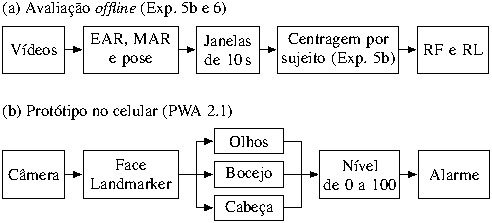
\includegraphics{fig_pipeline.pdf}
\caption{Cadeias de processamento. (a) Avaliação \emph{offline} dos Exp.~5b e 6, com o mesmo extrator (Face Mesh do MediaPipe) e as mesmas características nas três bases; a centragem por sujeito só é usada no Exp.~5b, e o Exp.~6 usa as características brutas. (b) Protótipo no celular (PWA \AppVersao): olhos, bocejo e cabeça somam pontos num nível de 0 a 100, que dispara o alarme a partir de 70.}
\label{fig:pipeline}
\end{figure}

\subsection{Sinais, piscadas e características}
Usamos o Face Mesh do MediaPipe~\cite{kartynnik2019,lugaresi2019}, na versão 0.10.21, que fornece 468 pontos do rosto por quadro. Deles calculamos o EAR~\cite{soukupova2016}, que soma as duas alturas do olho e divide o total pelo dobro da largura, com a média dos dois olhos; a abertura da boca dividida pela largura (MAR); e a pose da cabeça. O olho conta como fechado quando o EAR fica abaixo de 0,75 vezes a mediana do EAR na referência do sujeito (Seção~\ref{sec:rotulos}), e daí saem as piscadas e os fechamentos de 0,5\,s ou mais. Contra a anotação quadro a quadro das \SinaisDetectorSessoes{} sessões s5 do DMD, esse detector tem F1 de piscadas de \SinaisDetectorFUmPiscadas{} e, por quadro, $\kappa$ de Cohen de \SinaisDetectorKappaQuadro{} (médias por sessão); o fator 0,75 foi fixado antes dessa validação.

Nos Exp.~1, 2 e 5a, cada piscada é descrita pelas quatro características de~\cite{ghoddoosian2019}: duração, amplitude, velocidade de abertura e frequência acumulada. Normalizadas por \emph{z-score} do sujeito, elas formam sequências de 30 piscadas com passo 2, de modo que sequências vizinhas dividem 28 piscadas. Nos Exp.~5b e 6, a unidade é a janela de 10\,s com passo de 5\,s, descrita por 11 características que não dependem da taxa de quadros: PERCLOS, taxa de piscadas, duração média da piscada, maior fechamento, número de fechamentos de 0,5\,s ou mais, média e desvio do EAR, amplitude e velocidade médias das piscadas, fração do tempo em bocejo (MAR acima de 0,5 por 1\,s ou mais) e fração de quadros com rosto. A nota de um vídeo é a média das notas das suas janelas.

\subsection{Rótulos, normalização e modelos}
\label{sec:rotulos}
No DMD, uma janela é sonolenta se pertence à s5 e contém um fechamento anotado de 0,5\,s ou mais ou um bocejo, e é alerta se está inteira num trecho de direção segura da s2. As janelas da s5 sem evento anotado ficam de fora, porque são ambíguas. Na UTA-RLDD, o rótulo é o do vídeo, e o esquema principal, B3, compara alerta (KSS de 1 a 3) com sonolento (KSS 8 e 9), como no DMD. Cada característica é centrada por sujeito: subtraímos a média de uma referência separada, que nunca entra na avaliação. Ela é a direção segura da s3 no DMD e o último terço do vídeo alerta na UTA-RLDD, como no código original. O \emph{z-score} completo não é estimável em boa parte dos sujeitos do DMD, que têm poucas janelas de referência. Os classificadores são um Random Forest (RF) com 300 árvores e uma regressão logística (RL) com padronização, ambos com classes balanceadas, valores ausentes preenchidos pela mediana do treino e hiperparâmetros fixados antes. No Exp.~1, o RF usa 24 estatísticas de cada sequência, seis por característica, e uma LSTM de 32 unidades usa a sequência bruta. O estágio ocular usa uma CNN compacta própria, a EyeNet (diferente da homônima de~\cite{rahman2020}), com \ExpTresParametros{} parâmetros e recortes de 48$\times$48 em tons de cinza, exportada em TFLite fp32 e int8.

\subsection{Protótipo móvel}
\label{sec:app}
O protótipo é uma aplicação web progressiva (PWA, versão \AppVersao) que roda no navegador do celular, sem enviar vídeo. O Face Landmarker do MediaPipe fornece 478 pontos, 52 \emph{blendshapes} e a pose da cabeça, e três sinais visíveis são calibrados em 10\,s com a pessoa olhando para a frente:
\begin{itemize}
\item \textbf{olhos}: fechados quando os dois \emph{eyeBlink} ficam altos ou quando o EAR cai abaixo de 0,75 do valor da calibração, com regras de exclusão para olhar para baixo, olhos apertados e olhar lateral. Fechamentos de 0,5 a 1\,s somam pontos, e olhos fechados por 1\,s ou mais (microssono) levam ao vermelho imediatamente. O PERCLOS de 60\,s conta só fechamentos de 0,5\,s ou mais;
\item \textbf{bocejo}: \emph{jawOpen} ou MAR acima do repouso por 1,5\,s ou mais;
\item \textbf{cabeça}: queda (cabeça 18$^\circ$ abaixo do repouso por 0,8\,s) ou cabeceio, sempre \emph{com os olhos fechados}. Cabeça baixa com os olhos abertos conta como distração e não soma pontos.
\end{itemize}
Os eventos somam pontos que decaem com o tempo num nível de 0 a 100. O estado passa a amarelo em 40 e a vermelho em 70, com histerese, e o vermelho toca uma sirene. Os pontos de um único sinal não chegam a 70; o microssono e a cabeça caída com os olhos fechados levam direto ao vermelho. A LSTM do Exp.~1 soma no máximo 10 pontos, e a CNN do Exp.~3 só é exibida. Os pesos do nível são escolhas de projeto documentadas, não ajustadas em sonolência real, mas a regra dos olhos e os ajustes finais foram escolhidos nos dados da validação (Seção~\ref{sec:valapp}). A versão 1.0, substituída, alarmava por olho fechado, por um PERCLOS que contava piscadas ou pela LSTM sozinha.

% =====================================================================
\section{Protocolo Experimental}
\label{sec:prot}

A PP1 é respondida pelo Exp.~5b, com três cenários: A, DMD$\rightarrow$DMD, deixando um sujeito de fora; B, UTA$\rightarrow$UTA, nos 5 \emph{folds} oficiais; e C, DMD$\rightarrow$UTA. A queda da PP1 é B$-$C. Os Exp.~1 (reprodução do protocolo oficial), 2 (vazamento) e 5a (troca de extrator) apoiam a PP1; o Exp.~4 responde à PP2; e os Exp.~3 (estado ocular) e 6 (noite e movimento), à PP3. A área sob a curva ROC (AUC, $\times$100) mede a ordenação sem depender de limiar; a acurácia balanceada usa o limiar 0,5, fixado antes, e um limiar calibrado só com o treino. Os intervalos de confiança de 95\% (IC\,95\%) vêm de \emph{bootstrap} percentil sobre sujeitos (1.000 reamostragens), pareado na queda B$-$C; numa análise adicional, os motoristas do DMD também são reamostrados, e C é treinado de novo a cada reamostragem. O Exp.~5a usa também permutação pareada por sujeito. No Exp.~6, a relação sinal-ruído (SNR) do EAR é a amplitude das piscadas dividida pelo ruído quadro a quadro, medido como o desvio robusto em torno de uma mediana móvel de 1\,s; a taxa de disparo é a fração de janelas marcadas como sonolentas e, como o NITYMED não tem classe alerta, não é acurácia. A semente é 42 em todos os experimentos, e as partições aleatórias usam 42, 43 e 44. Cada número de resultado sai dos arquivos CSV do repositório por um \emph{script} que registra arquivo, coluna e filtro, e um segundo \emph{script} recalcula todos eles a partir desses arquivos.

% =====================================================================
\section{Resultados}
\label{sec:res}

\subsection{PP1: da sonolência atuada para a real (Exp.~5b)}
\label{sec:respp1}
A Fig.~\ref{fig:exp5b} resume o experimento central. Na AUC por janela, o RF obtém \ExpCincoBAUCJanelaAComIC{} no DMD (A) e \ExpCincoBAUCJanelaBComIC{} na UTA-RLDD quando treinado nela (B). Treinado só no DMD e aplicado à UTA-RLDD (C), fica em \ExpCincoBAUCJanelaCComIC, acima do acaso. A queda B$-$C é de \ExpCincoBQuedaAUCJanelaComIC{} pontos de AUC por janela e de \ExpCincoBQuedaAUCVideoComIC{} por vídeo (B: \ExpCincoBAUCVideoB; C: \ExpCincoBAUCVideoC). A RL repete o padrão, com queda de \ExpCincoBLRQuedaAUCJanelaComIC{} por janela e de \ExpCincoBLRQuedaAUCVideoComIC{} por vídeo.

\begin{figure}[t]
\centering
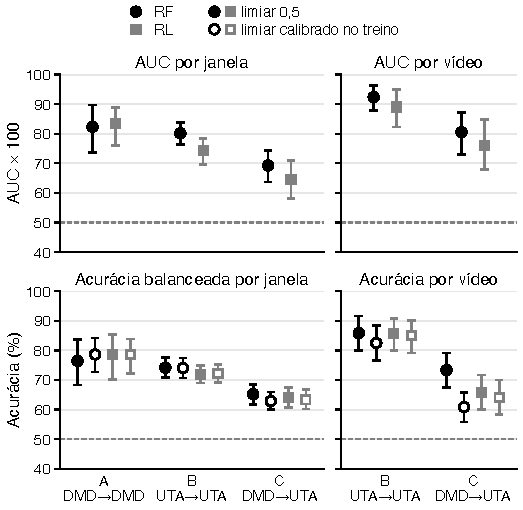
\includegraphics[width=\columnwidth]{fig_exp5b_transferencia.pdf}
\caption{Exp.~5b: AUC e acurácia por janela e por vídeo nos cenários A (DMD$\rightarrow$DMD), B (UTA$\rightarrow$UTA) e C (DMD$\rightarrow$UTA), com IC\,95\% por \emph{bootstrap} de sujeitos; esquema B3 na UTA-RLDD (\BaseUTASujeitos{} sujeitos, 5 \emph{folds} oficiais) e \BaseDMDSujeitos{} motoristas no DMD. Marcador cheio: limiar 0,5; vazado: limiar calibrado só no treino. A linha tracejada marca o acaso; o DMD (A) não tem nível de vídeo.}
\label{fig:exp5b}
\end{figure}

O modelo do DMD erra sobretudo ao chamar de alerta a sonolência real. No limiar 0,5, ele reconhece \ExpCincoBCEspecJanela\% das janelas alertas e só \ExpCincoBCSensJanela\% das sonolentas, e o limiar calibrado no DMD (\ExpCincoBLimiarCal) agrava o desequilíbrio (\ExpCincoBCSensJanelaCal\% das sonolentas e \ExpCincoBCEspecJanelaCal\% das alertas). As características brutas ajudam a entender o erro. Do alerta ao sonolento, a mediana do maior fechamento vai de \ExpCincoBMedianaFechMaxAlertaDMD{} a \ExpCincoBMedianaFechMaxSonolentoDMD\,s no DMD e de \ExpCincoBMedianaFechMaxAlertaUTA{} a \ExpCincoBMedianaFechMaxSonolentoUTA\,s na UTA-RLDD, e a do PERCLOS vai de \ExpCincoBMedianaPERCLOSAlertaDMD{} a \ExpCincoBMedianaPERCLOSSonolentoDMD{} e de \ExpCincoBMedianaPERCLOSAlertaUTA{} a \ExpCincoBMedianaPERCLOSSonolentoUTA. A sonolência atuada aparece bem mais intensa que a real, em parte por construção, já que as janelas sonolentas do DMD são as que contêm um evento anotado e as da UTA-RLDD são todas as do vídeo sonolento.

\begin{table}[t]
\centering
\caption{Exp.~5b: queda B$-$C da AUC (pontos), com IC\,95\%, sob controles da normalização e do treino; por janela, salvo onde indicado. Na configuração principal, a referência da UTA-RLDD é o último terço do vídeo alerta e a do DMD é a s3. Na última linha, mediana de 20 sorteios, sem IC.}
\label{tab:controles}
\scriptsize
\setlength{\tabcolsep}{3pt}
\begin{tabularx}{\columnwidth}{@{}>{\raggedright\arraybackslash}X cc@{}}
\toprule
\textbf{Variação} & \textbf{RF} & \textbf{RL} \\
\midrule
Principal & \ExpCincoBQuedaAUCJanelaComIC & \ExpCincoBLRQuedaAUCJanelaComIC \\
IC com os motoristas do DMD reamostrados & \ExpCincoBBootDuploQuedaAUCJanelaIC & \ExpCincoBLRBootDuploQuedaAUCJanelaIC \\
UTA-RLDD: referência no vídeo de pouca vigilância & \ExpCincoBRefAltQuedaAUCJanelaComIC & \ExpCincoBLRRefAltQuedaAUCJanelaComIC \\
DMD: referência na s2 & \ExpCincoBRefSDoisQuedaAUCJanelaComIC & \ExpCincoBLRRefSDoisQuedaAUCJanelaComIC \\
Sem centragem & \ExpCincoBSemNormQuedaAUCJanelaComIC & \ExpCincoBLRSemNormQuedaAUCJanelaComIC \\
Sem centragem, por vídeo & \ExpCincoBSemNormQuedaAUCVideoComIC & \ExpCincoBLRSemNormQuedaAUCVideoComIC \\
Contraste KSS 8 e 9 $\times$ 6 e 7 & \ExpCincoBControleQuedaCincoDezComIC & \ExpCincoBLRControleQuedaCincoDezComIC \\
B treinado com 13 sujeitos & \ExpCincoBTrezeQuedaAUCJanela & \ExpCincoBLRTrezeQuedaAUCJanela \\
\bottomrule
\end{tabularx}
\end{table}

A Tabela~\ref{tab:controles} mostra quanto da queda resiste aos controles. Na UTA-RLDD, as janelas alertas saem do mesmo vídeo usado como referência da normalização, e o RF treinado nela aproveita essa semelhança. Quando a referência vem do vídeo de pouca vigilância (KSS 6 e 7), que não entra na avaliação, ou quando não há centragem, a AUC de B no RF cai de \ExpCincoBAUCJanelaB{} para \ExpCincoBRefAltAUCJanelaB{} e \ExpCincoBSemNormAUCJanelaB, e a queda deixa de ser detectável; nessa variante, o limiar de EAR do detector continua o do vídeo alerta. Entre dois vídeos que não são a referência, a queda não é detectável em nenhum dos dois modelos, e por vídeo, sem centragem, também não. Na RL, a queda por janela fica entre \ExpCincoBLRQuedaNormMin{} e \ExpCincoBLRQuedaNormMax{} pontos nas quatro normalizações testadas, sempre com IC acima de zero. O volume do treino explica pouco: com 13 sujeitos da UTA-RLDD por \emph{fold}, como no DMD, a queda continua clara nos dois modelos. Reamostrar também os motoristas do DMD alarga o IC da queda principal, que fica acima de zero. Usar como alerta do DMD a direção com o carro em movimento (s1) piora a transferência (AUC de C de \ExpCincoBAUCJanelaC{} para \ExpCincoBAlertaSUmAUCJanelaC). Nas variações de janela (5 e 15\,s), de alerta e de referência no DMD e na exclusão do motorista em que o detector falhou, o IC da queda do RF fica acima de zero; contando a principal e a sem centragem, são \ExpCincoBSensVariantesICPositivo{} de \ExpCincoBSensVariantesTotal{} variantes.

\subsection{Protocolo, reprodução e extrator (Exp.~1, 2 e 5a)}
A Tabela~\ref{tab:exp12} reúne os números de referência. No protocolo oficial, o RF sobre 24 estatísticas das piscadas empata com a HM-LSTM na acurácia por sequência (BSA, do inglês \emph{blink sequence accuracy}) e fica \ExpUmDifHMLSTMRFVA\,pp abaixo na acurácia por vídeo (VA), no nível do julgamento humano. Sem a classe intermediária (B3), chega à acurácia balanceada de \ExpUmRFBTresAcBal\% (acaso: 50\%), com a mesma estrutura de referência discutida acima. Repartir as mesmas sequências por janela, com janelas do mesmo vídeo nos dois lados, infla a BSA em \ExpDoisRFInflacaoJanelaBSA\,pp no RF e \ExpDoisLSTMInflacaoJanelaBSA\,pp na LSTM; como sequências vizinhas dividem 28 das 30 piscadas, o teste vê quase as mesmas sequências do treino. A partição por vídeo, em que o treino tem os outros vídeos do mesmo sujeito com rótulos diferentes, fica \emph{abaixo} da partição por sujeito (\ExpDoisRFInflacaoVideoBSA\,pp); uma explicação provável, que não isolamos, é que o modelo associa o padrão de piscadas da pessoa a rótulos que não são os do vídeo de teste. Nesta base, o que infla a acurácia é o mesmo vídeo, e com ele o mesmo rótulo, aparecer nos dois lados. No cenário do Exp.~5b, com janelas de 10\,s e duas classes, a partição aleatória de janelas infla a acurácia balanceada em \ExpCincoBVazamentoAcBal\,pp no RF e em só \ExpCincoBLRVazamentoAcBal\,pp na RL: o vazamento pesa nos modelos flexíveis, capazes de memorizar janelas vizinhas.

\begin{table}[t]
\centering
\caption{Exp.~1 e 2, três classes (\%): 5 \emph{folds} oficiais (média $\pm$ dp) e as mesmas sequências sob três partições. BSA: acurácia por sequência de 30 piscadas; VA: por vídeo; n/a: não se aplica. Referências de~\cite{ghoddoosian2019}.}
\label{tab:exp12}
\scriptsize
\setlength{\tabcolsep}{3pt}
\begin{tabular}{@{}llcc@{}}
\toprule
\textbf{Modelo} & \textbf{Partição} & \textbf{BSA} & \textbf{VA} \\
\midrule
RF (24 estatísticas) & 5 \emph{folds} oficiais & \ExpUmRFBSAMDP & \ExpUmRFVAMDP \\
LSTM (30$\times$4) & 5 \emph{folds} oficiais & \ExpUmLSTMBSAMDP & \ExpUmLSTMVAMDP \\
HM-LSTM~\cite{ghoddoosian2019} & 5 \emph{folds} oficiais & \ExpUmHMLSTMBSA & \ExpUmHMLSTMVA \\
Humanos~\cite{ghoddoosian2019} & n/a & n/a & \ExpUmHumanosVA \\
Classe majoritária & n/a & \ExpUmChanceBSA & \ExpUmChanceVA \\
\midrule
RF & por janela & \ExpDoisRFJanelaBSA & n/a \\
RF & por vídeo & \ExpDoisRFVideoBSA & \ExpDoisRFVideoVA \\
RF & por sujeito & \ExpDoisRFSujeitoBSA & \ExpDoisRFSujeitoVA \\
LSTM & por janela & \ExpDoisLSTMJanelaBSA & n/a \\
LSTM & por sujeito & \ExpDoisLSTMSujeitoBSA & \ExpDoisLSTMSujeitoVA \\
\bottomrule
\end{tabular}
\end{table}

Trocar o extrator dos autores (dlib) pelo nosso (MediaPipe), com o RF treinado nas características oficiais, custa \ExpCincoACustoAcBalDifComIC\,pp de acurácia balanceada em três classes (\emph{p}\,=\,\ExpCincoACustoAcBalP; \ExpCincoASujeitos{} sujeitos, \ExpCincoAVideos{} vídeos), custo que não se distingue de zero. Com cada extrator no próprio treino e teste, o nosso separa melhor alerta de sonolento nos 5 \emph{folds} (oficial menos nosso em B3: \ExpCincoAMesmoBTresAcBalDifComIC\,pp; \emph{p}\,=\,\ExpCincoAMesmoBTresAcBalP), mas essa vantagem não se distingue de zero quando se deixa um sujeito de fora por vez (\ExpCincoAMesmoLOSOBTresAcBalDifComIC\,pp). Não há, portanto, perda detectável ao trocar de extrator, embora o IC largo não prove equivalência; com essa ressalva, usamos o nosso nas duas pontas do Exp.~5b.

\subsection{PP2: custo no celular (Exp.~4)}
\label{sec:respp2}
A Tabela~\ref{tab:exp4} reúne as medidas. A CNN do olho cai de \ExpQuatroCNNFloatKB{} para \ExpQuatroCNNIntKB\,KB em int8, com perda de no máximo \ExpQuatroQuedaQuantizacaoMax\,pp, e a LSTM exportada concorda com o modelo original em Keras em \ExpUmLSTMConcordancia\% das sequências. No iPhone~17~Pro (\CelularIPhoneSistema, \CelularIPhoneNavegador, Face Landmarker na \CelularIPhoneDelegate), \CelularIPhoneExecucoes{} execuções de 60\,s da versão \CelularIPhoneVersaoApp{} do app somaram \CelularIPhoneQuadros{} quadros, \CelularIPhoneTaxaRosto\% deles com rosto, e o tempo total por quadro (p50) ficou entre \CelularIPhoneTotalPcinquentaMin{} e \CelularIPhoneTotalPcinquentaMax\,ms nas execuções, dominado pelo Face Landmarker.\ifSamsungMedido{} No Galaxy S23 Ultra (\CelularSamsungSistema, \CelularSamsungNavegador), \CelularSamsungExecucoes{} execuções da versão \CelularSamsungVersaoApp{} ficaram entre \CelularSamsungTotalPcinquentaMin{} e \CelularSamsungTotalPcinquentaMax\,ms por quadro.\fi{} O iPhone registra os tempos em milissegundos inteiros, o que limita a precisão dos estágios mais rápidos. Numa execução da versão 1.0, com um dos autores acordado diante da câmera, a lógica antiga acusou PERCLOS de \CelularVUmFalsoAlarmePERCLOS\% e manteve o alarme ligado em \CelularVUmFalsoAlarmeFracao\% dos quadros; esse falso alarme motivou a reescrita descrita na Seção~\ref{sec:app}.

\begin{table}[t]
\centering
\caption{Exp.~4. (a) Modelos e quantização. (b) Tempo por quadro na PWA (versão \CelularIPhoneVersaoApp{} do app), em ms: mediana, entre as execuções de 60\,s, do p50 e do p95 de cada execução.}
\label{tab:exp4}
\scriptsize
\setlength{\tabcolsep}{3pt}
\begin{tabular}{@{}lr@{}}
\multicolumn{2}{@{}l}{\textbf{(a) Modelos}}\\
\toprule
CNN do olho: fp32 $\rightarrow$ int8 (KB) & \ExpQuatroCNNFloatKB{} $\rightarrow$ \ExpQuatroCNNIntKB \\
Maior perda de acurácia com int8 (pp) & \ExpQuatroQuedaQuantizacaoMax \\
LSTM: parâmetros / tamanho (KB) & \ExpUmLSTMParametros{} / \ExpUmLSTMKB \\
\bottomrule
\end{tabular}

\vspace{3pt}
\ifSamsungMedido
\begin{tabular}{@{}lcc@{}}
\multicolumn{3}{@{}l}{\textbf{(b) \emph{Pipeline} completo, CNN int8 (p50 / p95)}}\\
\toprule
\textbf{Estágio} & \textbf{iPhone 17 Pro} & \textbf{Galaxy S23 Ultra} \\
\midrule
Face Landmarker & \CelularIPhoneLandmarkerPcinquenta{} / \CelularIPhoneLandmarkerPnoventaecinco & \CelularSamsungLandmarkerPcinquenta{} / \CelularSamsungLandmarkerPnoventaecinco \\
CNN, 2 olhos & \CelularIPhoneCNNPcinquenta{} / \CelularIPhoneCNNPnoventaecinco & \CelularSamsungCNNPcinquenta{} / \CelularSamsungCNNPnoventaecinco \\
LSTM & \CelularIPhoneLSTMPcinquenta{} / \CelularIPhoneLSTMPnoventaecinco & \CelularSamsungLSTMPcinquenta{} / \CelularSamsungLSTMPnoventaecinco \\
Motor de sinais & \CelularIPhoneMotorPcinquenta{} / \CelularIPhoneMotorPnoventaecinco & \CelularSamsungMotorPcinquenta{} / \CelularSamsungMotorPnoventaecinco \\
Total por quadro & \CelularIPhoneTotalPcinquenta{} / \CelularIPhoneTotalPnoventaecinco & \CelularSamsungTotalPcinquenta{} / \CelularSamsungTotalPnoventaecinco \\
\bottomrule
\end{tabular}
\else
\begin{tabular}{@{}lc@{}}
\multicolumn{2}{@{}l}{\textbf{(b) \emph{Pipeline} completo, CNN int8 (p50 / p95)}}\\
\toprule
\textbf{Estágio} & \textbf{iPhone 17 Pro} \\
\midrule
Face Landmarker & \CelularIPhoneLandmarkerPcinquenta{} / \CelularIPhoneLandmarkerPnoventaecinco \\
CNN, 2 olhos & \CelularIPhoneCNNPcinquenta{} / \CelularIPhoneCNNPnoventaecinco \\
LSTM & \CelularIPhoneLSTMPcinquenta{} / \CelularIPhoneLSTMPnoventaecinco \\
Total por quadro & \CelularIPhoneTotalPcinquenta{} / \CelularIPhoneTotalPnoventaecinco \\
\bottomrule
\end{tabular}
\fi
\end{table}

\subsection{PP3: condições de captura (Exp.~3 e 6)}
\begin{figure*}[t]
\centering
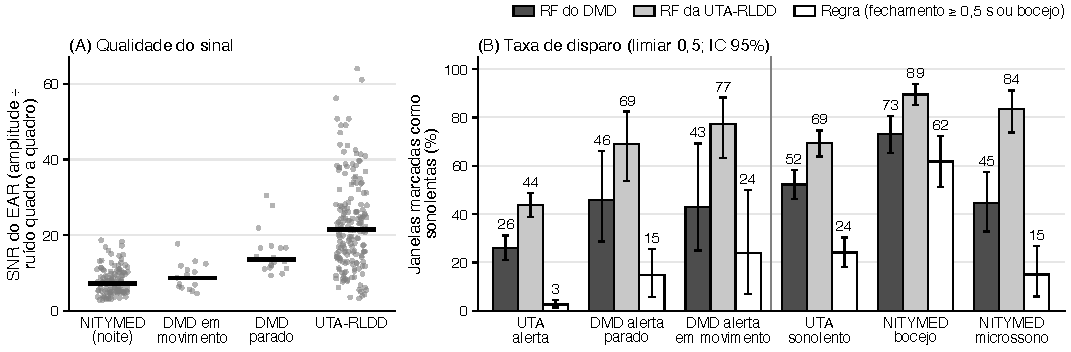
\includegraphics[width=\textwidth]{fig_exp6_noite.pdf}
\caption{Exp.~6, com características brutas, pois o NITYMED não tem trecho alerta para a referência. (A) SNR do EAR por vídeo (traço = mediana); o DMD é de dia, com o carro em movimento ou parado. (B) Fração de janelas de 10\,s marcadas como sonolentas no limiar 0,5 pelo RF do DMD, pelo RF da UTA-RLDD e pela regra de fechamento de 0,5\,s ou mais ou bocejo, com IC\,95\%; a linha vertical separa os grupos de pessoas acordadas dos sonolentos e noturnos. No próprio domínio, os valores são fora da amostra (UTA-RLDD: 5 \emph{folds}; DMD parado: um motorista de fora por vez); no DMD em movimento, os motoristas estão no treino com outras sessões. Nenhum valor no NITYMED é acurácia.}
\label{fig:exp6}
\end{figure*}
No estado ocular, a EyeNet atinge \ExpTresIntraMRLAcMDP\% em sujeitos não vistos do MRL, \ExpTresMRLCEWPatchAcMDP\% do MRL para o CEW (média dos \emph{folds}; \ExpTresFinalMRLCEWPatchAc\% com o modelo treinado em todos os sujeitos) e \ExpTresCEWPatchMRLAcMDP\% do CEW para o MRL. Do CEW para o MRL, a AUC cai com óculos (\ExpTresCEWPatchMRLComOculosAUC{} contra \ExpTresCEWPatchMRLSemOculosAUC{} sem óculos), pouca luz (\ExpTresCEWPatchMRLIlumRuimAUC{} contra \ExpTresCEWPatchMRLIlumBoaAUC) e reflexo grande (\ExpTresCEWPatchMRLReflexoGrandeAUC{} contra \ExpTresCEWPatchMRLSemReflexoAUC); na acurácia balanceada, a queda aparece com óculos (\ExpTresCEWPatchMRLComOculosAcBal\% contra \ExpTresCEWPatchMRLSemOculosAcBal\%) e pouca luz (\ExpTresCEWPatchMRLIlumRuimAcBal\% contra \ExpTresCEWPatchMRLIlumBoaAcBal\%), mas não com reflexo. Essas condições estão ligadas entre si e aos sujeitos, e as diferenças devem ser lidas como associações.

À noite, o rosto continua sendo encontrado em \ExpSeisRostoNoite\% dos quadros do NITYMED, contra \ExpSeisRostoUTA\% na UTA-RLDD (diferença de \ExpSeisDifRostoNoiteUTAComIC\,pp). O que cai é a qualidade do sinal (Fig.~\ref{fig:exp6}A): a SNR do EAR é de \ExpSeisSNRNoiteComIC{} no NITYMED, contra \ExpSeisSNRUTA{} na UTA-RLDD e \ExpSeisSNRDMDParado{} no DMD parado. Mas os mesmos motoristas do DMD, de dia e com o carro em movimento, ficam em \ExpSeisSNRDMDMovimento. No mesmo motorista e com a mesma câmera, o movimento muda a SNR em \ExpSeisDifSNRMovimentoParadoComIC{} (\ExpSeisSujeitosPareadosMovimento{} motoristas), e a diferença entre a noite e o carro em movimento não se distingue de zero (\ExpSeisDifSNRNoiteDMDMovimentoComIC). Com estes dados, a perda de sinal acompanha a condução real, e um efeito adicional da escuridão não é detectável. Sem um trecho alerta do próprio motorista, como o da calibração do protótipo, o PERCLOS também não separa microssono de ruído de condução: com o limiar tirado do próprio vídeo, sua mediana sobe tanto nos vídeos de microssono do NITYMED (\ExpSeisPERCLOSMicrossonoPNoventa\%) quanto nos motoristas acordados do DMD em movimento (\ExpSeisPERCLOSDMDMovimentoPNoventa\%).

Na Fig.~\ref{fig:exp6}B, sem centragem, que o NITYMED não permite por falta de trecho alerta, os dois RF marcam como sonolentas de \ExpSeisDisparoModeloDMDUTAAlerta\% a \ExpSeisDisparoModeloUTAUTAAlerta\% das janelas de pessoas acordadas da UTA-RLDD no limiar 0,5. A regra do rótulo do DMD aplicada aos nossos sinais (fechamento de 0,5\,s ou mais, com o limiar de EAR do próprio sujeito, ou bocejo) marca \ExpSeisDisparoRegraUTAAlerta\% (\ExpSeisDisparoRegraUTAAlertaIC). Com o limiar calibrado no treino, o RF do DMD dispara ainda menos (\ExpSeisDisparoModeloDMDCalUTAAlerta\%), mas encontra menos janelas sonolentas que a regra (\ExpSeisDisparoModeloDMDCalUTASonolento\% contra \ExpSeisDisparoRegraUTASonolento\%); a RL do DMD, no limiar 0,5, marca \ExpSeisDisparoModeloDMDLRUTAAlerta\% e \ExpSeisDisparoModeloDMDLRUTASonolento\%. Com o carro em movimento, o RF calibrado e a regra disparam em \ExpSeisDisparoModeloDMDCalDMDMovimento\% e \ExpSeisDisparoRegraDMDMovimento\% das janelas de motoristas acordados. Nos vídeos de microssono do NITYMED, o disparo do modelo do DMD (\ExpSeisDisparoModeloDMDMicrossono\%) fica no nível do disparo em motoristas acordados do DMD e não informa sensibilidade.

Nos vídeos, os óculos só puderam ser observados no DMD (\ExpCincoBMotoristasOculos{} motoristas), porque a UTA-RLDD não indica quais vídeos os têm. O detector falhou em um deles (F1 de piscadas de \ExpCincoBOculosFalhaFUm), em que o EAR cai só \ExpCincoBOculosFalhaQuedaEAR\% ao fechar o olho, contra \ExpCincoBSemOculosQuedaEARMin\% a \ExpCincoBSemOculosQuedaEARMax\% sem óculos; com um caso em três, a falha não pode ser atribuída aos óculos.

\subsection{Validação do protótipo}
\label{sec:valapp}
A Tabela~\ref{tab:app} resume a versão \AppVersao. Contra a anotação do DMD, a combinação de EAR e \emph{blendshape} marca o olho fechado com $\kappa$ de \AppKappaOffline{} por quadro, contra \AppKappaEARSozinho{} do EAR sozinho. O bocejo com a mão na boca quase nunca é detectado (\AppBocejoAcertosComMao{} de \AppBocejoAnotadosComMao); no navegador, foram \AppBocejosNavegadorAcertos{} de \AppBocejosNavegadorAnotados{}, todos entre os \AppBocejosNavegadorAnotadosSemMao{} sem a mão. Em \AppDMDMinutosDirecaoReal\,min de direção real com motoristas acordados (sessões s1 do DMD), todo o vermelho veio de um motorista (\AppGACincoVermelho\% do tempo da sessão dele), cujo olhar para baixo o \emph{blendshape} lê como olho fechado. No navegador, com vídeos reais no lugar da câmera, só \AppUTASonolentoComVermelho{} dos \AppUTASonolentoVideos{} vídeos sonolentos da UTA-RLDD chegou ao vermelho. A queda da cabeça não tem revocação medida, pois o DMD não anota cabeceio; há só um teste sintético, com o vídeo girado, e casos isolados. Uma ressalva vale para toda a tabela: a regra dos olhos e os ajustes da versão \AppVersao{} foram escolhidos comparando variantes nessas mesmas sessões e clipes, e os números são, portanto, de desenvolvimento, não de um teste independente.

\begin{table}[t]
\centering
\caption{Validação do protótipo (PWA \AppVersao). Motor \emph{offline} no DMD, com o mesmo Face Landmarker e o mesmo código do app: s5 = sonolência encenada com anotação; s1 = direção real com motoristas acordados. Navegador: Chrome com vídeos reais no lugar da câmera. Verde, amarelo e vermelho são os estados do nível.}
\label{tab:app}
\scriptsize
\setlength{\tabcolsep}{3pt}
\begin{tabularx}{\columnwidth}{@{}>{\raggedright\arraybackslash}X r@{}}
\toprule
\textbf{Medida} & \textbf{Valor} \\
\midrule
Olho fechado por quadro, $\kappa$ (s5): \emph{offline} / navegador & \AppKappaOffline{} / \AppKappaNavegador \\
Fechamentos de 1\,s ou mais (s5): revocação / precisão & \AppFechUmSRevocacao{} / \AppFechUmSPrecisao \\
Bocejos (s5): revocação sem mão / com mão & \AppBocejoRevocacaoSemMao{} / \AppBocejoRevocacaoComMao \\
Bocejos falsos em s1 & \AppDMDBocejosFalsosDirecaoReal \\
Tempo em vermelho em s1 (\%): versão \AppVersao{} / lógica 1.0 & \AppDMDVermelhoDirecaoReal{} / \AppDMDVermelhoVUmDirecaoReal \\
Sessões de s1 sem alarme & \AppDMDSessoesSemAlarme{} de \AppDMDSessoesDirecaoReal \\
Tempo em vermelho em s5 (\%) & \AppDMDVermelhoSonolencia \\
Navegador, UTA-RLDD alerta (3 vídeos): tempo em verde (\%) / alarmes & \AppUTAAlertaVerdeMin{} / \AppUTAAlertaAlarmes \\
Navegador, UTA-RLDD sonolento: vídeos com vermelho & \AppUTASonolentoComVermelho{} de \AppUTASonolentoVideos \\
\bottomrule
\end{tabularx}
\end{table}

% =====================================================================
\section{Discussão}
\label{sec:disc}

\textbf{PP1.} Treinar no DMD em vez da UTA-RLDD custa AUC com o mesmo extrator e as mesmas características, mas o tamanho da perda depende do modelo e da normalização. Na RL, ela fica entre \ExpCincoBLRQuedaNormMin{} e \ExpCincoBLRQuedaNormMax{} pontos por janela nas quatro normalizações testadas. No RF, os \ExpCincoBQuedaAUCJanela{} pontos da configuração principal vêm em boa parte de B aproveitar a semelhança entre as janelas alertas e a referência tirada do mesmo vídeo; com outra referência na UTA-RLDD ou sem centragem, a diferença fica entre \ExpCincoBQuedaOutrasNormMin{} e \ExpCincoBQuedaOutrasNormMax{} pontos e não é detectável. Num app, a calibração e a sonolência acontecem na mesma sessão, e essa vantagem de B não se repetiria. O padrão de erro é estável: o modelo do DMD aprende com eventos longos e deixa passar a sonolência real, de fechamentos curtos e PERCLOS baixo. Com um único par de bases, a queda ainda se mistura com a câmera, o cenário e a natureza do rótulo, que no DMD é um evento encenado e na UTA-RLDD é o estado relatado.

No mesmo cenário, o vazamento por janelas do mesmo vídeo infla a acurácia balanceada do RF em \ExpCincoBVazamentoAcBal\,pp, mais que a queda B$-$C (\ExpCincoBQuedaAcBalJanela\,pp, que depende da referência); na RL, infla \ExpCincoBLRVazamentoAcBal\,pp, contra uma queda de \ExpCincoBLRQuedaAcBalJanela\,pp. O protocolo pesa muito nos modelos capazes de memorizar janelas vizinhas e pouco no modelo linear. Os 90\% de~\cite{lyu2018,shen2020}, porém, foram medidos com pessoas que não estavam no treino, e a distância até a UTA-RLDD não se explica por esse vazamento. Separar vídeos que não são a referência continua difícil: entre KSS 8 e 9 e KSS 6 e 7, a AUC fica em \ExpCincoBControleAUCCincoDezB{} mesmo com o RF treinado na UTA-RLDD.

\textbf{PP2.} O custo no celular é pequeno: \CelularIPhoneTotalPcinquenta\,ms por quadro no iPhone~17~Pro\ifSamsungMedido{} e \CelularSamsungTotalPcinquenta\,ms no Galaxy S23 Ultra\fi, dominado pelo rastreador facial. Os modelos aprendidos ocupam \ExpQuatroCNNIntKB\,KB (CNN int8) e \ExpUmLSTMKB\,KB (LSTM), e a quantização custa no máximo \ExpQuatroQuedaQuantizacaoMax\,pp. A resposta vale para a PWA no navegador, \ifSamsungMedido em dois aparelhos de topo\else num aparelho de topo\fi{} e em execuções de 60\,s; não medimos bateria, aquecimento em uso longo nem aparelhos de entrada.

\textbf{PP3.} A degradação não é uniforme: no estado ocular, a AUC entre bases cai com óculos, pouca luz e reflexo grande, e o detector de piscadas falhou num dos \ExpCincoBMotoristasOculos{} motoristas de óculos do DMD. À noite, a captura do rosto quase não muda, mas a SNR do EAR cai para \ExpSeisSNRNoite; de dia, os mesmos motoristas do DMD vão de \ExpSeisSNRDMDParado{} a \ExpSeisSNRDMDMovimento{} com o carro em movimento. Parte da degradação atribuída à noite vem, portanto, do movimento, provavelmente da vibração, dos movimentos de cabeça e da luz variável, embora a comparação com o NITYMED não isole a escuridão (limitação 3). No limiar 0,5, os RF com características brutas disparam em muitas janelas de pessoas acordadas, e a regra sobre sinais visíveis em poucas, mas esse limiar é arbitrário. Escolhendo, só para comparar, o limiar que dá o falso alarme da regra nas janelas alertas, a RL do DMD com centragem encontra tantas janelas sonolentas quanto ela (\ExpCincoBLROpRegraSensCCentrada\% contra \ExpSeisDisparoRegraUTASonolento\%), e os outros modelos do DMD encontram menos (\ExpCincoBOpRegraSensCBruta\% e \ExpCincoBLROpRegraSensCBruta\% com características brutas; \ExpCincoBOpRegraSensCCentrada\% no RF centrado). A regra não é mais precisa que os modelos; ela fica na mesma curva, sem treino e com cada alarme explicável. Isso, somado à transferência limitada da PP1, justifica o desenho do protótipo: regras interpretáveis calibradas por usuário, com o modelo aprendido só como reforço limitado. Nenhum dos dois resolve o carro em movimento, em que disparam em \ExpSeisDisparoModeloDMDCalDMDMovimento\% e \ExpSeisDisparoRegraDMDMovimento\% das janelas de motoristas acordados.

\textbf{Limitações.} (1)~Os rótulos têm naturezas diferentes: eventos encenados e anotados no DMD e KSS relatado para o vídeo inteiro na UTA-RLDD, com cada estado gravado em outro momento; o Exp.~5b mede também uma troca de pergunta. (2)~O DMD tem \BaseDMDSujeitos{} motoristas atuados (\BaseDMDJanelasAlerta{} janelas alertas), o carro parado nas sessões de treino e, na maioria dos sujeitos, o alerta gravado em outro dia; o tipo de sonolência continua misturado com a câmera e o cenário. (3)~O NITYMED não tem classe alerta nem identificação do motorista, o que deixa otimistas os IC por vídeo, e a noite vem junto com outra câmera, outra compressão e outras pessoas. (4)~O mapeamento entre sujeitos oficiais e pastas da UTA-RLDD, usado no Exp.~5a, é uma reconstrução nossa. (5)~\ifSamsungMedido Os dois aparelhos foram medidos em execuções curtas\else Só um aparelho foi medido, em \CelularIPhoneExecucoes{} execuções curtas\fi, e o aplicativo Android nativo do repositório não foi avaliado. (6)~A validação do protótipo usa sonolência atuada e poucos vídeos no navegador, os mesmos dados usados para escolher as regras; os pesos do nível não foram ajustados em sonolência real, há um falso alarme conhecido em direção real e a queda da cabeça não tem revocação medida. (7)~As análises de sensibilidade são descritivas, sem correção para comparações múltiplas, e o desenho não foi pré-registrado.

\textbf{Ética, LGPD e falsa segurança.} O protótipo processa o vídeo só no aparelho, o que evita enviar dados biométricos, tratados como sensíveis pela Lei Geral de Proteção de Dados (LGPD); as bases foram usadas segundo seus termos e nenhum rosto foi publicado. O sistema detecta sinais visíveis, não o estado interno: quem relata sono sem mostrar sinais não é detectado, como nos vídeos sonolentos da UTA-RLDD que não chegaram ao vermelho no navegador. Ele não é um dispositivo certificado, não diagnostica distúrbios do sono e não substitui o descanso previsto na Lei n\textsuperscript{o}~13.103/2015; a ausência de alarme não significa condutor alerta.

% =====================================================================
\section{Conclusão e Trabalhos Futuros}
\label{sec:conc}

Com o mesmo extrator nas duas bases, modelos treinados com sonolência atuada (DMD) reconhecem a sonolência real (UTA-RLDD) pior que modelos treinados nela. Por janela, a regressão logística perde de \ExpCincoBLRQuedaNormMin{} a \ExpCincoBLRQuedaNormMax{} pontos de AUC em todas as normalizações testadas; o Random Forest perde \ExpCincoBQuedaAUCJanela{} na principal, mas a diferença não é detectável com outra referência na UTA-RLDD. Os erros são compatíveis com uma sonolência atuada mais intensa que a real, mas parte da diferença vem da regra de rótulo do DMD e de diferenças entre as bases que este desenho não separa. O vazamento por trechos do mesmo vídeo infla a acurácia em até \ExpDoisRFInflacaoJanelaBSA\,pp nas sequências de piscadas e em \ExpCincoBVazamentoAcBal\,pp nas janelas do Exp.~5b, no RF. À noite, a perda de sinal ocular é compatível com a do carro em movimento. O protótipo segue essas evidências, com regras explicáveis sobre olhos, bocejo e cabeça, e a versão \CelularIPhoneVersaoApp{} processou cada quadro em \CelularIPhoneTotalPcinquenta\,ms num iPhone~17~Pro\ifSamsungMedido{} e em \CelularSamsungTotalPcinquenta\,ms num Galaxy S23 Ultra\fi. Na sonolência real, ele ainda deixa passar casos: só \AppUTASonolentoComVermelho{} dos \AppUTASonolentoVideos{} vídeos sonolentos testados no navegador chegou ao vermelho.

Como trabalhos futuros, propomos repetir a transferência com outra base de sonolência real, como o DROZY, e com a referência gravada na mesma sessão, como num app; validar o app em campo, com voluntários, KSS, óculos e noite; e medir a revocação da queda da cabeça.

\section*{Agradecimentos}
Trabalho da disciplina Experiência Criativa: Projeto Transformador II (turma 8\textsuperscript{o}A, equipe 14), orientado pelo Prof. Júlio César Nievola. Agradecemos aos autores da UTA-RLDD, do DMD e do NITYMED por disponibilizarem as bases. Ferramentas de IA generativa foram usadas como apoio na escrita do texto e do código; os autores conferiram todo o conteúdo e respondem por ele.

\bibliographystyle{IEEEtran}
\bibliography{refs}

\end{document}
